\documentclass[10pt, french]{article}
%% -----------------------------
%% Préambule
%% -----------------------------
% !TEX encoding = UTF-8 Unicode
% LaTeX Preamble for all cheatsheets
% Author : Gabriel Crépeault-Cauchon

% HOW-TO : copy-paste this file in the same directory as your .tex file, and add in your preamble the next command right after you have specified your documentclass : 
% \input{preamble-cheatsht.tex}
% ---------------------------------------------
% ---------------------------------------------

% Extra note : this preamble creates document that are meant to be used inside the multicols environment. See the documentation on internet for further information.

%% -----------------------------
%% Encoding packages
%% -----------------------------
\usepackage[utf8]{inputenc}
\usepackage[T1]{fontenc}
\usepackage{babel}
\usepackage{lmodern}

%% -----------------------------
%% Variable definition
%% -----------------------------
\def\auteur{Gabriel Crépeault-Cauchon / Nicholas Langevin}
\def\BackgroundColor{white}

%% -----------------------------
%% Margin and layout
%% -----------------------------
% Determine the margin for cheatsheet
\usepackage[landscape, hmargin=1cm, vmargin=1.7cm]{geometry}
\usepackage{multicol}

% Remove automatic indentation after section/subsection title.
\setlength{\parindent}{0cm}

% Save space in cheatsheet by removing space between align environment and normal text.
\usepackage{etoolbox}
\newcommand{\zerodisplayskips}{%
  \setlength{\abovedisplayskip}{0pt}%
  \setlength{\belowdisplayskip}{0pt}%
  \setlength{\abovedisplayshortskip}{0pt}%
  \setlength{\belowdisplayshortskip}{0pt}}
\appto{\normalsize}{\zerodisplayskips}
\appto{\small}{\zerodisplayskips}
\appto{\footnotesize}{\zerodisplayskips}

%% -----------------------------
%% URL and links
%% -----------------------------
\usepackage{hyperref}
\hypersetup{colorlinks = true, urlcolor = gray!70!white, linkcolor = black}

%% -----------------------------
%% Document policy (uncomment only one)
%% -----------------------------
%	\usepackage{concrete}
	\usepackage{mathpazo}
%	\usepackage{frcursive} %% permet d'écrire en lettres attachées
%	\usepackage{aeguill}
%	\usepackage{mathptmx}
%	\usepackage{fourier} 

%% -----------------------------
%% Math configuration
%% -----------------------------
\usepackage[fleqn]{amsmath}
\usepackage{amsthm,amssymb,latexsym,amsfonts}
\usepackage{empheq}
\usepackage{numprint}
\usepackage{dsfont} % Pour avoir le symbole du domaine Z

% Mathematics shortcuts

\newcommand{\reels}{\mathbb{R}}
\newcommand{\entiers}{\mathbb{Z}}
\newcommand{\naturels}{\mathbb{N}}
\newcommand{\eval}{\biggr \rvert}
\usepackage{cancel}
\newcommand{\derivee}[1]{\frac{\partial}{\partial #1}}
\newcommand{\prob}[1]{\Pr \left( #1 \right)}
\newcommand{\esp}[1]{\mathrm{E} \left[ #1 \right]} % espérance
\newcommand{\variance}[1]{\mathrm{Var} \left( #1   \right)}
\newcommand{\covar}[1]{\mathrm{Cov} \left( #1   \right)}
\newcommand{\laplace}{\mathcal{L}}
\newcommand{\deriv}[2][]{\frac{\partial^{#1}}{\partial #2^{#1}}}
\newcommand{\e}[1]{\mathrm{e}^{#1}}
\newcommand{\te}[1]{\text{exp}\left\{#1\right\}}
\DeclareMathSymbol{\shortminus}{\mathbin}{AMSa}{"39}



% To indicate equation number on a specific line in align environment
\newcommand\numberthis{\addtocounter{equation}{1}\tag{\theequation}}

%
% Actuarial notation packages
%
\usepackage{actuarialsymbol}
\usepackage{actuarialangle}

%
% Matrix notation for math symbols (\bm{•})
%
\usepackage{bm}
% Matrix notation variable (bold style)
\newcommand{\matr}[1]{\mathbf{#1}}



%% -----------------------------
%% tcolorbox configuration
%% -----------------------------
\usepackage[most]{tcolorbox}
\tcbuselibrary{xparse}
\tcbuselibrary{breakable}

%%
%% Coloured box "definition" for definitions
%%
\DeclareTColorBox{definition}{ o }				% #1 parameter
{
	colframe=blue!60!green,colback=blue!5!white, % color of the box
	breakable, 
	pad at break* = 0mm, 						% to split the box
	title = {#1},
	after title = {\large \hfill \faBook},
}
%%
%% Coloured box "definition2" for definitions
%%
\DeclareTColorBox{definitionNOHFILL}{ o }				% #1 parameter
{
	colframe=blue!60!green,colback=blue!5!white, % color of the box
	pad at break* = 0mm, 						% to split the box
	title = {#1},
	before title = {\faBook \quad },
	breakable
}


%%
%% Coloured box "algo" for algorithms
%%
\newtcolorbox{algo}[ 1 ]
{
	colback = blue!5!white,
	colframe = blue!75!black,
	title=#1,
	fonttitle = \bfseries,
	breakable
}
%%
%% Coloured box "conceptgen" for points adding to a concept's deifintion
%%
\newtcolorbox{conceptgen}[ 1 ]
{
	breakable,
	colback = beaublue,
	colframe = airforceblue,
	title=#1,
	fonttitle = \bfseries
}
%%
%% Coloured box "probch3" pour formules relatives au 3ème chapitre de prob
%%
\newtcolorbox{probch3}[ 1 ]
{
	colback = ruddypink,
	colframe = burgundy,
	fonttitle = \bfseries,	
	breakable,
	title=#1
}
%%
%% Coloured box "formula" for formulas
%%
\newtcolorbox{formula}[ 1 ]
{
	colback = green!5!white,
	colframe = green!70!black,
	breakable,
	fonttitle = \bfseries,
	title=#1
}
%%
%% Coloured box "formula" for formulas
%%
\DeclareTColorBox{algo2}{ o }
{
	enhanced,
	title = #1,
	colback=blue!5!white,	
	colbacktitle=blue!75!black,
	fonttitle = \bfseries,
	breakable,
	boxed title style={size=small,colframe=arsenic} ,
	attach boxed title to top center = {yshift=-3mm,yshifttext=-1mm},
}
%%
%% Coloured box "examplebox" for formulas
%%
\newtcolorbox{examplebox}[ 1 ]
{
	colback = lightmauve,
	colframe = antiquefuchsia,
	breakable,
	fonttitle = \bfseries,title=#1
}
%%
%% Coloured box "rappel" pour rappel de formules
%%
\newtcolorbox{rappel}[ 1 ]
{
	colback = ashgrey,
	colframe = arsenic,
	breakable,
	fonttitle = \bfseries,title=#1
}
%%
%% Coloured box "rappel" pour rappel de formules
%%
\DeclareTColorBox{rappel_enhanced}{ o }
{
	enhanced,
	title = #1,
	colback=ashgrey, % color of the box
%	colframe=blue(pigment),
%	colframe=arsenic,	
	colbacktitle=arsenic,
	fonttitle = \bfseries,
	breakable,
	boxed title style={size=small,colframe=arsenic} ,
	attach boxed title to top center = {yshift=-3mm,yshifttext=-1mm},
}
%%
%% Coloured box "notation" for notation and terminology
%%
\DeclareTColorBox{distributions}{ o }			% #1 parameter
{
	enhanced,
	title = #1,
	colback=gray(x11gray), % color of the box
%	colframe=blue(pigment),
	colframe=arsenic,	
	colbacktitle=aurometalsaurus,
	fonttitle = \bfseries,
	boxed title style={size=small,colframe=arsenic} ,
	attach boxed title to top center = {yshift=-3mm,yshifttext=-1mm},
	breakable
%	left=0pt,
%  	right=0pt,
%    box align=center,
%    ams align*
%  	top=-10pt
}

%% -----------------------------
%% Graphics and pictures
%% -----------------------------
\usepackage{graphicx}
\usepackage{pict2e}
\usepackage{tikz}

%% -----------------------------
%% insert pdf pages into document
%% -----------------------------
\usepackage{pdfpages}

%% -----------------------------
%% Color configuration
%% -----------------------------
\usepackage{color, soulutf8, colortbl}


%
%	Colour definitions
%
\definecolor{blue(munsell)}{rgb}{0.0, 0.5, 0.69}
\definecolor{blue(matcha)}{rgb}{0.596, 0.819, 1.00}
\definecolor{blue(munsell)-light}{rgb}{0.5, 0.8, 0.9}
\definecolor{bleudefrance}{rgb}{0.19, 0.55, 0.91}
\definecolor{blizzardblue}{rgb}{0.67, 0.9, 0.93}
\definecolor{bondiblue}{rgb}{0.0, 0.58, 0.71}
\definecolor{blue(pigment)}{rgb}{0.2, 0.2, 0.6}
\definecolor{bluebell}{rgb}{0.64, 0.64, 0.82}
\definecolor{airforceblue}{rgb}{0.36, 0.54, 0.66}
\definecolor{beaublue}{rgb}{0.74, 0.83, 0.9}
\definecolor{cobalt}{rgb}{0.0, 0.28, 0.67}	% nice light blue-ish
\definecolor{blue_rectangle}{RGB}{83, 84, 244}		% ACT-2004
\definecolor{indigo(web)}{rgb}{0.29, 0.0, 0.51}	% purple-ish
\definecolor{antiquefuchsia}{rgb}{0.57, 0.36, 0.51}	%	pastel dark purple ish
\definecolor{darkpastelpurple}{rgb}{0.59, 0.44, 0.84}
\definecolor{gray(x11gray)}{rgb}{0.75, 0.75, 0.75}
\definecolor{aurometalsaurus}{rgb}{0.43, 0.5, 0.5}
\definecolor{ruddypink}{rgb}{0.88, 0.56, 0.59}
\definecolor{pastelred}{rgb}{1.0, 0.41, 0.38}		
\definecolor{lightmauve}{rgb}{0.86, 0.82, 1.0}
\definecolor{azure(colorwheel)}{rgb}{0.0, 0.5, 1.0}
\definecolor{darkgreen}{rgb}{0.0, 0.2, 0.13}			
\definecolor{burntorange}{rgb}{0.8, 0.33, 0.0}		
\definecolor{burntsienna}{rgb}{0.91, 0.45, 0.32}		
\definecolor{ao(english)}{rgb}{0.0, 0.5, 0.0}		% ACT-2003
\definecolor{amber(sae/ece)}{rgb}{1.0, 0.49, 0.0} 	% ACT-2004
\definecolor{green_rectangle}{RGB}{131, 176, 84}		% ACT-2004
\definecolor{red_rectangle}{RGB}{241,112,113}		% ACT-2004
\definecolor{amethyst}{rgb}{0.6, 0.4, 0.8}
\definecolor{amethyst-light}{rgb}{0.6, 0.4, 0.8}
\definecolor{ashgrey}{rgb}{0.7, 0.75, 0.71}			% dark grey-black-ish
\definecolor{arsenic}{rgb}{0.23, 0.27, 0.29}			% light green-beige-ish gray
\definecolor{amaranth}{rgb}{0.9, 0.17, 0.31}
\definecolor{brickred}{rgb}{0.8, 0.25, 0.33}
\definecolor{pastelred}{rgb}{1.0, 0.41, 0.38}

%
% Useful shortcuts for coloured text
%
\newcommand{\orange}{\textcolor{orange}}
\newcommand{\red}{\textcolor{red}}
\newcommand{\cyan}{\textcolor{cyan}}
\newcommand{\blue}{\textcolor{blue}}
\newcommand{\green}{\textcolor{green}}
\newcommand{\purple}{\textcolor{magenta}}
\newcommand{\yellow}{\textcolor{yellow}}

%% -----------------------------
%% Enumerate environment configuration
%% -----------------------------
%
% Custum enumerate & itemize Package
%
\usepackage{enumitem}
%
% French Setup for itemize function
%
\frenchbsetup{StandardItemLabels=true}
%
% Change default label for itemize
%
\renewcommand{\labelitemi}{\faAngleRight}


%% -----------------------------
%% Tabular column type configuration
%% -----------------------------
\newcolumntype{C}{>{$}c<{$}} % math-mode version of "l" column type
\newcolumntype{L}{>{$}l<{$}} % math-mode version of "l" column type
\newcolumntype{R}{>{$}r<{$}} % math-mode version of "l" column type
\newcolumntype{f}{>{\columncolor{green!20!white}}p{1cm}}
\newcolumntype{g}{>{\columncolor{green!40!white}}m{1.2cm}}
\newcolumntype{a}{>{\columncolor{red!20!white}$}p{2cm}<{$}}	% ACT-2005
% configuration to force a line break within a single cell
\usepackage{makecell}


%% -----------------------------
%% Fontawesome for special symbols
%% -----------------------------
\usepackage{fontawesome}

%% -----------------------------
%% Section Font customization
%% -----------------------------
\usepackage{sectsty}
\sectionfont{\color{\SectionColor}}
\subsectionfont{\color{\SubSectionColor}}

%% -----------------------------
%% Footer/Header Customization
%% -----------------------------
\usepackage{lastpage}
\usepackage{fancyhdr}
\pagestyle{fancy}

%
% Header
%
\fancyhead{} 	% Reset
\fancyhead[L]{Aide-mémoire pour~ \cours ~(\textbf{\sigle})}
\fancyhead[R]{\auteur}

%
% Footer
%
\fancyfoot{}		% Reset
\fancyfoot[R]{\thepage ~de~ \pageref{LastPage}}
\fancyfoot[L]{\href{https://github.com/ressources-act/Guide_de_survie_en_actuariat}{\faGithub \ ressources-act/Guide de survie en actuariat}}
%
% Page background color
%
\pagecolor{\BackgroundColor}




%% END OF PREAMBLE
% ---------------------------------------------
% ---------------------------------------------
%% -----------------------------
%% Variable definition
%% -----------------------------
\def\cours{Apprentissage statistique en actuariat}
\def\sigle{ACT-3114}
%% -----------------------------
%% Colour setup for sections
%% -----------------------------
\def\SectionColor{green!50!black}
\def\SubSectionColor{green!20!black}
\def\SubSubSectionColor{burntsienna}

%	"to-do" list
\newlist{todolist}{itemize}{2}
\setlist[todolist]{label=$\square$}
%%%
\definecolor{ballblue}{rgb}{0.13, 0.67, 0.8}
\definecolor{darkgreen}{rgb}{0.0, 0.2, 0.13}
\definecolor{rstudioblue}{HTML}{F7F7F7}


%% -----------------------------
%% Début du document
%% -----------------------------
\begin{document}

\begin{center}
	\textsc{\Large Contributeurs}\\[0.5cm] 
\end{center}
\begin{contrib}{ACT-3114\: Apprentissage statistique en actuariat}
\begin{description}
	\item[aut., cre.] Alec James van Rassel
	\item[src.] Marie-Pier Côté
\end{description}
\end{contrib}

\newpage

\raggedcolumns
\begin{multicols*}{3} 

\section{Préparation de données}

\begin{algo2}[Repères visuels]
\begin{enumerate}[leftmargin = *]
	\item	La \textbf{position} sur une \textbf{même échelle} (variable numérique), souvent à l’aide de points ou de boîte à moustache;
	\item	La \textbf{position} sur une \textbf{échelle identique}, mais \textbf{non alignée} (variable numérique);
		\begin{itemize}
		\item	Pour exemple, lorsqu’on utilise des facettes.
		\end{itemize}
	\item	La \textbf{longueur} sur une \textbf{même échelle} (variable numérique);
		\begin{itemize}
		\item	Pour exemple, dans un diagramme à bande ou un histogramme.
		\end{itemize}
	\item	L’angle ou \textbf{la pente} (variable numérique);
		\begin{itemize}
		\item	Pour exemple, en représentant les données sous forme de lignes (pente);
		\item	Pour exemple, la redoutable pointe à tarte (angle).
		\end{itemize}
	\item	La \textbf{forme des points} (variable catégorielle) peut représenter le groupe;
	\item	L’aire ou \textbf{le volume} (variable numérique);
		\begin{itemize}
		\item	Pour exemple, dans un diagramme à bande ou un histogramme;
		\end{itemize}
	\item	La \textbf{saturation de la couleur} (numérique ou catégorielle) peut représenter “à quel point” sur une échelle de claire à foncé;
		\begin{itemize}
		\item	Pour exemple, gris vs noir.
		\end{itemize}
	\item	La \textbf{teinte de couleur} (numérique ou catégorielle).
		\begin{itemize}
		\item	Pour exemple, bleu vs rouge.
		\end{itemize}
\end{enumerate}
\end{algo2}

\begin{algo2}[Étapes du nettoyage de données]
Cette liste n'est pas séquentielle, il est surtout important de \textit{tout} le faire.
\begin{todolist}[leftmargin = *]
	\item	\textbf{Comprendre} la structure des données;
		\begin{itemize}[leftmargin = *]
		\item	dimensions, types de variables, \texttt{str} et \texttt{summary}.
		\end{itemize}
	\item	\textbf{Visualiser} les données;
		\begin{itemize}[leftmargin = *]
		\item	\texttt{head}, \texttt{summary} et graphiques exploratoires.
		\end{itemize}
	\item	\textbf{Mettre en forme \textit{(format)}} les données;
		\begin{itemize}[leftmargin = *]
		\item	Chaque ligne est une observation;
		\item	Chaque colonne est une variable;
		\item	Supprimer les doublons;
		\end{itemize}
	\item	Vérifier et corriger les \textbf{types} de variables;
		\begin{itemize}[leftmargin = *]
		\item	booléens, entiers, numériques, facteurs, chaînes de caractères, dates, etc.
		\end{itemize}
	\item	\textbf{Manipuler} les \textbf{chaînes} de caractères;
		\begin{itemize}[leftmargin = *]
		\item	Corriger les typos;
		\item	Changer la casse avec \texttt{tolower};
		\item	Extraire des informations avec les expressions régulières.
		\end{itemize}
	\item	Identifier les \textbf{données aberrantes};
		\begin{itemize}[leftmargin = *]
		\item	Mettre \texttt{NA} et gérer plus tard.
		\end{itemize}
	\item	\textbf{Détecter} les \textbf{erreurs} flagrantes ou les changements structurels dans les données;
		\begin{itemize}[leftmargin = *]
		\item	Prendre compte des réformes;
		\item	Constater les structures importantes.
		\end{itemize}
	\item	\textbf{Augmenter} les données à l'aide d'autres sources;
		\begin{itemize}[leftmargin = *]
		\item	optionnel.
		\end{itemize}
\end{todolist}
\end{algo2}

\begin{conceptgen}{Types de variables}
Les jeux de données peuvent être:
\begin{description}[leftmargin = *]
	\item[Structuré:]	Données ayant une structure prédéfinie.\\
		Pour exemple:
		\begin{itemize}[leftmargin = *]
		\item	Tableaux;
		\item	\og spreadsheet \fg{};
		\item	\og Relational databases \fg{}.
		\end{itemize}
	\item[Non structuré:]	Données sans structure prédéfinie venant en toute forme et ne pouvant pas être facilement résumées à un tableau.\\
		Pour exemple:
		\begin{multicols*}{3}
		\begin{itemize}[leftmargin = *]
		\item	Texte;
		\item	Images;
		\item	Audio;
		\end{itemize}
		\end{multicols*}
\end{description}
\begin{center}
	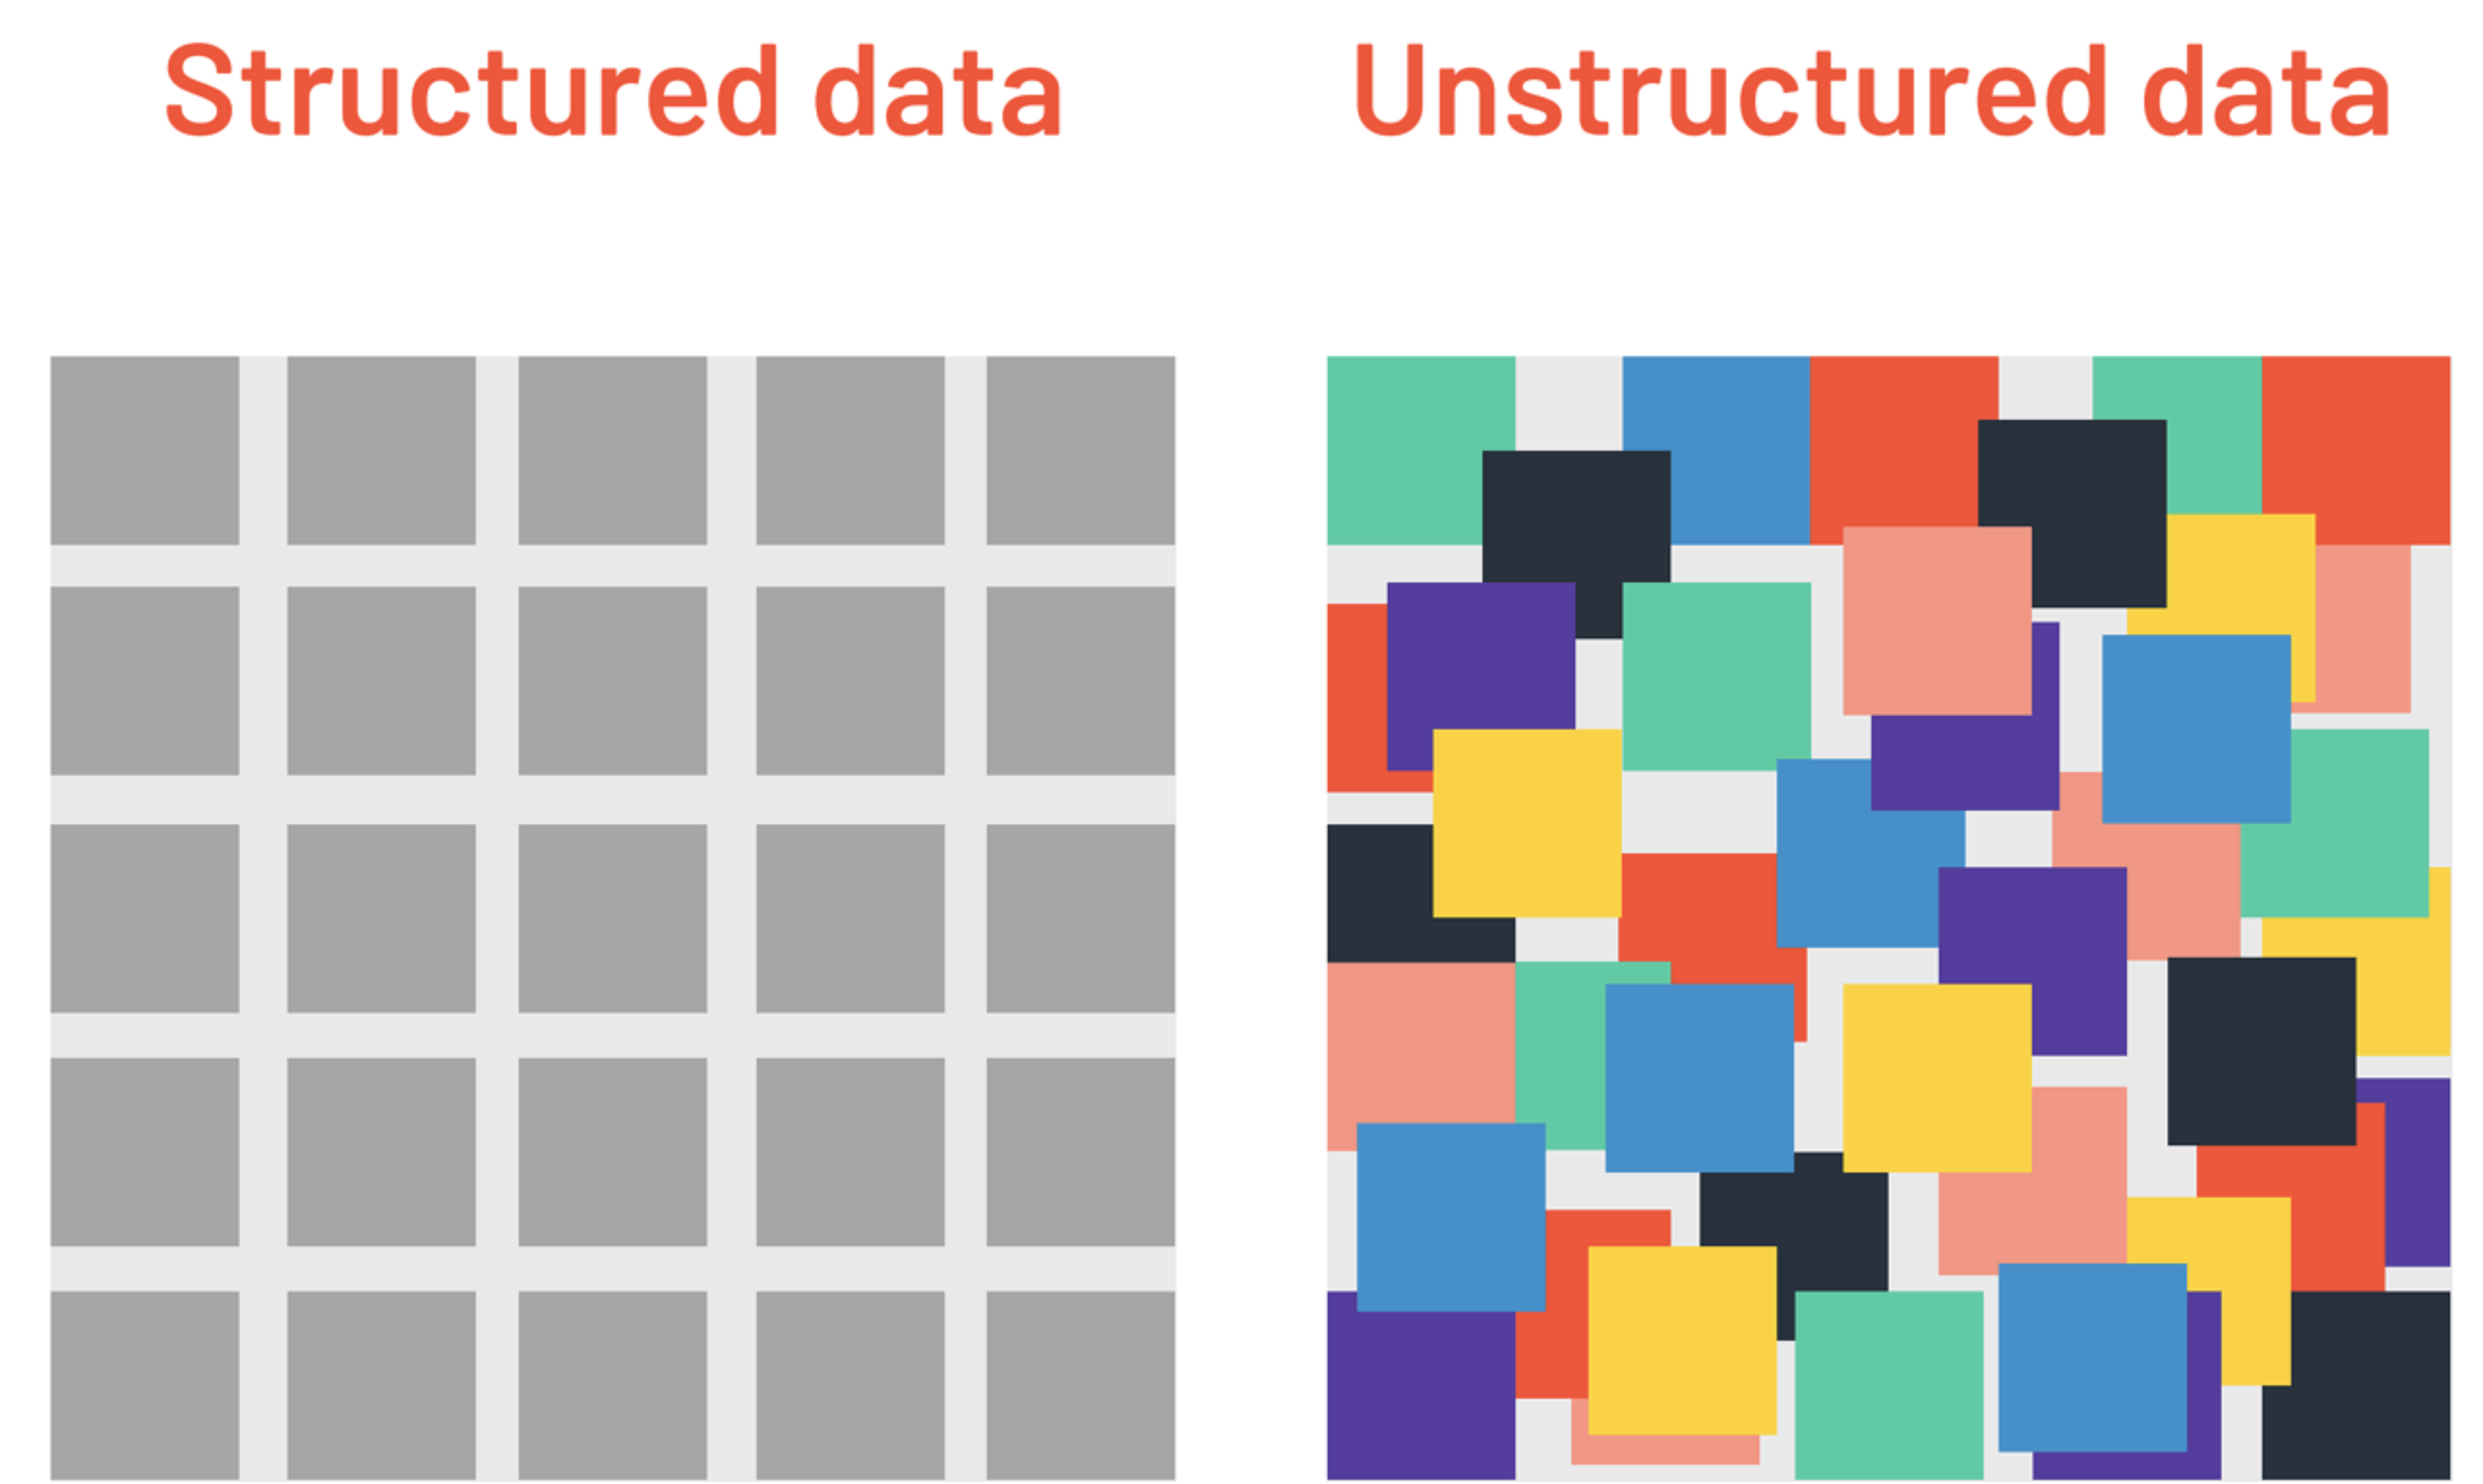
\includegraphics[scale=0.15]{src/ACT-3114/data-un-structured.png}
\end{center}

Types de variables:
\begin{description}
	\item[Quantitatives:]	Données numériques pouvant être:
		\begin{itemize}[leftmargin = *]
		\item	Discrète, pour exemple des données de comptage; 
		\item	Continue, pour exemple des montants de sinistre.
		\end{itemize}
	\item[Qualitatives:]	Données catégorielles pouvant être:
		\begin{itemize}[leftmargin = *]
		\item	Nominales, pour exemple le sexe; 
		\item	Ordinales, pour exemple des groupes d'âge.
		\end{itemize}
	\item[Temporelles]Données chronologiques représentant un état dans le temps;
		\begin{itemize}[leftmargin = *]
		\item	Pour exemple, la quantité totale de pluie au Canada le 1er juillet 1990.
		\end{itemize}
	\item[Spatiales]	Données géographiques avec des coordonnées (pour exemple, la latitude et longitude).
\end{description}
\end{conceptgen}

\begin{algo2}[Conseils]
\begin{itemize}[leftmargin = *]
	\item	Conserver un script séparé pour le traitement des données;
	\item	Documenter nos choix;
		\begin{itemize}[leftmargin = *]
		\item	Si l'on omet quelques observations en raison de données aberrantes, il faut être conscients que ça peut biaiser les résultats.
		\end{itemize}
	\item	Effacer l'encre superflue 
	
	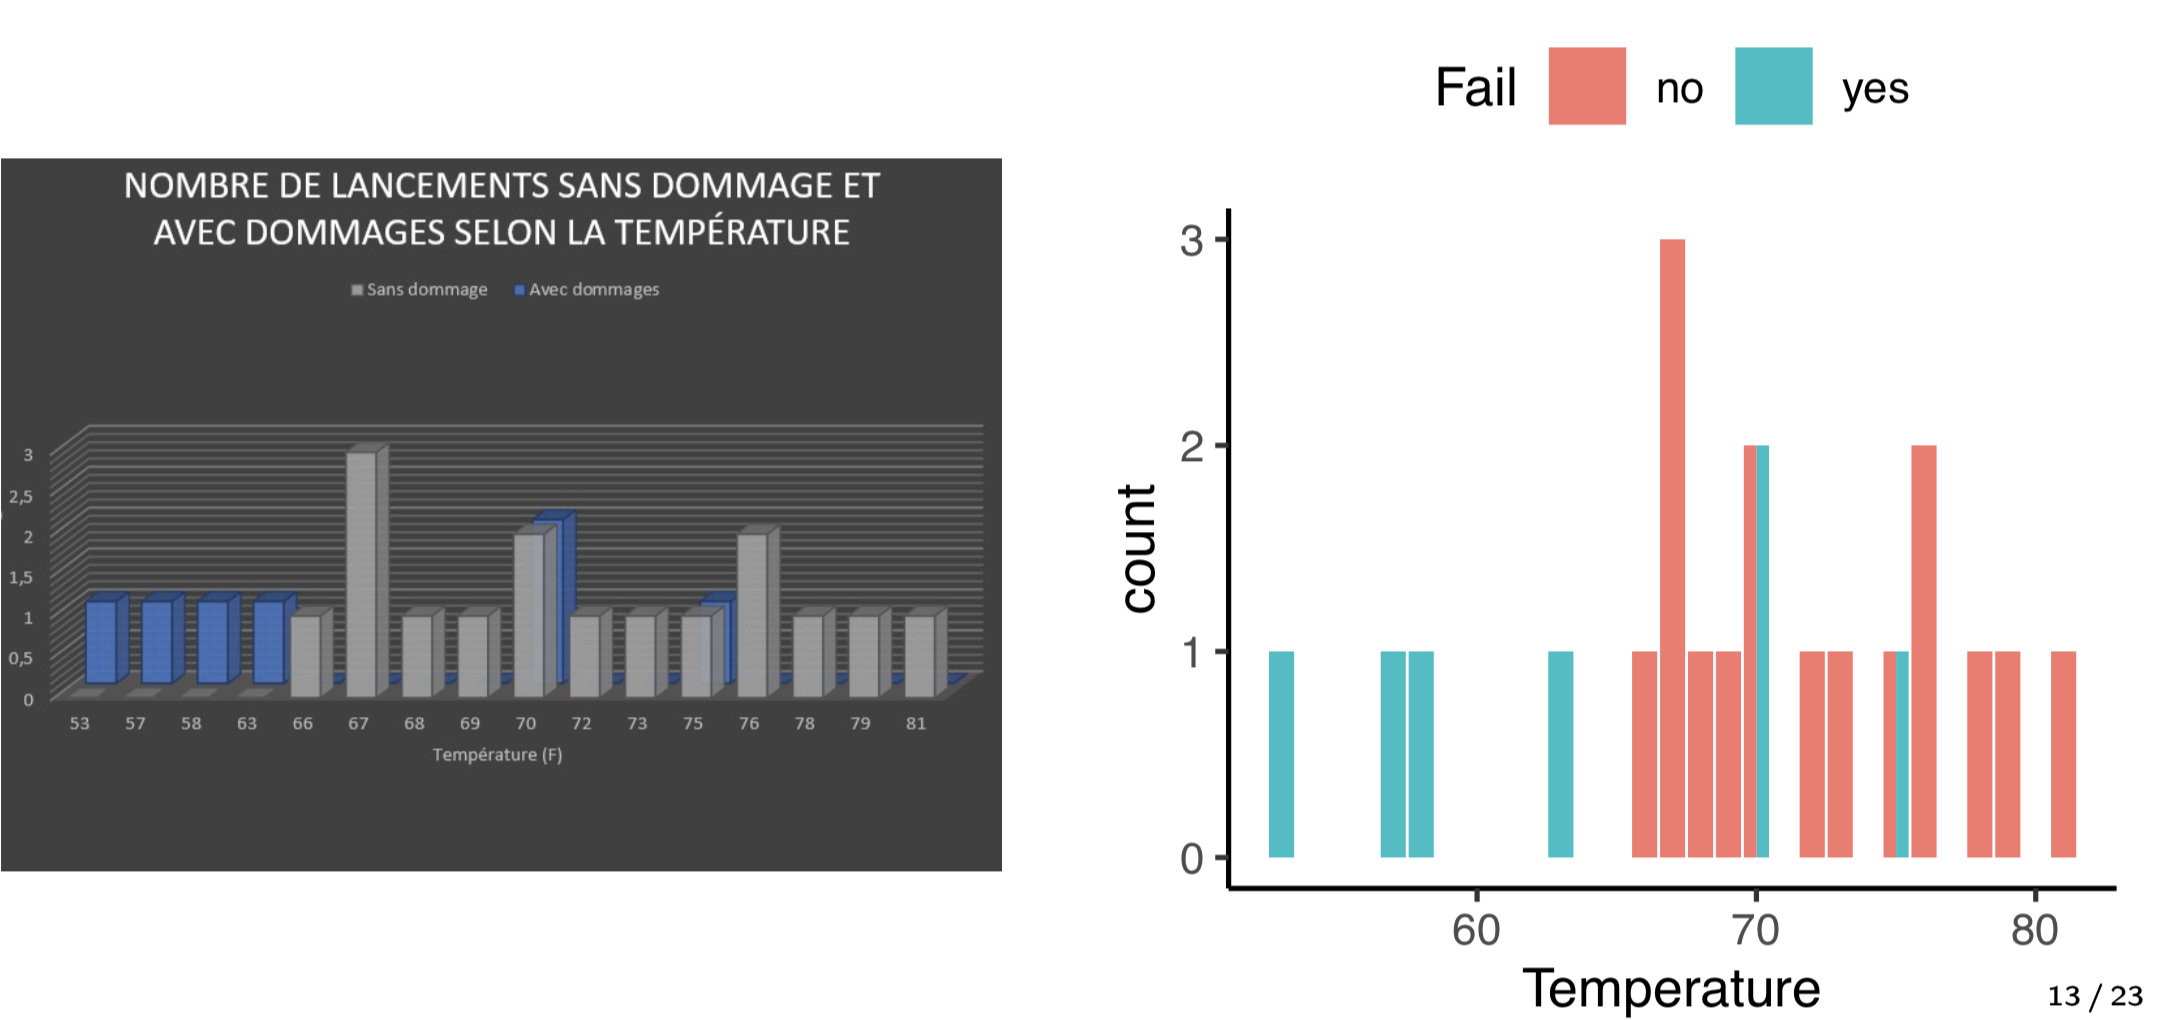
\includegraphics[scale=0.15]{src/ACT-3114/data-superfluous.png}
	\item	Considérer l'étique:
		\begin{itemize}[leftmargin = *]
		\item	Avons-nous l'autorisation d'utiliser les données?
		\item[]	Pour exemple, les données ouvertes du gouvernement avec peu de restrictions;
		\item	Est-ce qu'il y a des considérations éthiques à l'utilisation des données?
		\item[]	Pour exemple, Facebook qui utilise les données de façon immorale;
		\item	Est-ce qu'il y a des biais dans les données pouvant causer préjudice?
		\item[]	Pour exemple, des données avec un biais sexiste ou raciste, des données financées par une compagnie.
		\end{itemize}
\end{itemize}
\end{algo2}

\begin{conceptgen}{Biais}
\begin{description}
	\item[d'échantillonnage]	Lorsque les données d'entraînement ne représentent pas de façon représentative la vraie population.\\
		Pour exemple:
		\begin{itemize}[leftmargin = *]
		\item	Entraîner une voiture autonome seulement le jour alors qu'elles peuvent être conduites jour et soir;
		\item	Sonder les lecteurs du Devoir sur le parti pour lequel ils vont voter à l'élection et donc ignorer ceux ne lisant pas le journal.
		\end{itemize}
	\item[de stéréotypes]	Données influencées par des stéréotypes (consciemment ou pas).\\
		Pour exemple:
		\begin{itemize}[leftmargin = *]
		\item	Entraîner un algorithme pour comprendre comment les personnes travaillent avec des images d'hommes sur des ordinateurs et de femmes à la maison;
		\item	L'algorithme aura tendance à penser que les hommes sont des programmeurs et les femmes des cuisinières.
		\end{itemize}
	\item[de mesure]	Données influencées par un problème avec l'instrument de mesure.\\
		Pour exemple:
		\begin{itemize}[leftmargin = *]
		\item	Entraîner un algorithme de reconnaissance d'image avec des images d'une caméra avec un filtre de couleur;
		\item	L'algorithme serait fondé sur des images ayant systématique mal-représentée le vrai environnement.
		\end{itemize}
	\item[de modèle]	Le compromis de biais-variance $B(\hat{\theta}) = \text{E}[\hat{\theta}] - \theta$.\\
		Pour exemple:
		\begin{itemize}[leftmargin = *]
		\item	Certaines variables ne sont pas considérées (ou mesurées);
		\item	Le modèle n'est pas assez flexible (compromis linéaire vs lisse)
		\end{itemize}
\end{description}
\end{conceptgen}

\newpage

\section{Données manquantes}

Le chapitre utilise la \textbf{mise en contexte} suivante:
\begin{itemize}[leftmargin = *]
	\item	Il y a une réclamation pour un accident d'auto en Ontario;
	\item	Le contrat d'assurance couvre les frais médicaux;
	\item	On désire calculer la probabilité de paiement (variable réponse) en fonction de:
		\begin{enumerate}[leftmargin = *]
		\item	La gravité de l'accident (variable explicative);
		\item[]	3 niveaux: mineur-majeur-catastrophique;
		\item	La souffrance du réclamant;
		\item[]	Échelle de 1 (peu) à 5 (beaucoup);
		\end{enumerate}
\end{itemize}

\textbf{Problèmes} de modélisation:
\begin{itemize}[leftmargin = *]
	\item	Comment analyser les données malgré les valeurs manquantes?
	\item	Quels enjeux ou problèmes devrait-on considérer dans la modélisation?
\end{itemize}

\subsection*{Terminologie}

\begin{definition}[Notation]
\begin{itemize}[leftmargin = *]
	\item[$Y_{ij}$:] Valeur de la variable explicative $j$ pour l'observation $i$ où	$j \in \left\{ 1, \dots, p \right\}$ et $i \in \{1, \dots, n\}$;
	\item[$\matr{Y}_{n \times p}$:] Matrice contenant les données \textbf{complètes};
	\item[]	$\matr{Y}$ est partitionné en deux, $\matr{Y} = \left\{ \matr{Y}_{obs}, \matr{Y}_{mis} \right\}$
		\begin{itemize}[leftmargin = *]
		\item[$\matr{Y}_{obs}$:] matrice avec les données ayant toutes les valeurs observées;
		\item[$\matr{Y}_{mis}$:] matrice avec les données comportant des valeurs manquantes;
		\end{itemize}
	\item[$\matr{R}_{n \times p}$:]	\textbf{Matrice de réponse} des variables indicatrices $R_{ij} = \matr{1}_{\{Y_{ij} \text{ observé}\}}$;
	\item[$\theta$:] \textbf{Paramètre de nuisance}
\end{itemize}
\end{definition}

\begin{examplebox}{Exemple de notation}
\begin{align*}
	\bm{Y}	
	&=	\begin{bmatrix}
		2	&	3	\\
		8	&	6	\\
		3	&	12	
		\end{bmatrix}	\\
	\bm{Y}_{obs}
	&=	\begin{bmatrix}
		2	&	.	\\
		8	&	6	\\
		.	&	.
		\end{bmatrix}	&
	\bm{Y}_{mis}
	&=	\begin{bmatrix}
		.	&	3	\\
		.	&	.	\\
		3	&	12	
		\end{bmatrix}	\\
	\bm{R}
	&=	\begin{bmatrix}
		1	&	0	\\
		1	&	1	\\
		0	&	0	
		\end{bmatrix}	
\end{align*}
\end{examplebox}

\subsection*{Mécanisme de non-réponse}
La distribution de $\matr{R}$ est le \textit{mécanisme de non-réponse};

\textbf{Types de données manquantes}:
\begin{enumerate}[leftmargin = *]
	\item	\textbf{MCAR}: Missing Completely at Random;
		\begin{itemize}[leftmargin = *]
		\item	Le patron de non-réponse (pattern of missing values) est indépendant des données $\matr{Y}$;
		\item	Il s'ensuit que la probabilité de réponse $f(R | \matr{Y}, \theta)$ ne dépend pas des données complètes $\matr{Y}$:
			\begin{align*}
			f(R | \matr{Y}, \theta) &= f(R | \theta) \\
			\end{align*}
%		\item	Pour example
		\begin{examplebox}{Exemple avec un $\theta$ de 10\%}
		On perd $10\%$ des valeurs mesurées alors, $\forall i \in \{1, \dots, n\}, j \in \{1, \dots, p\}$, la distribution du mécanisme de non-réponse:
		\setlength{\mathindent}{-1cm}
			\begin{align*}
			R_{ij} 
			&\sim 	\text{Bernoulli}(p = 1 - \theta =  90\%)
			\end{align*}
		\setlength{\mathindent}{1cm}
		\end{examplebox}
		\item	\textbf{Tester} la différence de moyennes:
		\end{itemize}	
		\setlength{\mathindent}{-2cm}
			\begin{align*}
			\mathcal{H}_{0}:
			&\left\{ p_{\text{Cat, mis}} - p_{\text{Cat, obs}} = 0 \right\} 
			\text{et}	\\
			&\left\{ p_{\text{Maj, mis}} - p_{\text{Maj, obs}} = 0 \right\}
			\end{align*}
		\setlength{\mathindent}{1cm}
		\begin{itemize}[leftmargin = *]
		\item[]	Est équivalent à tester: 
		\end{itemize}	
		\setlength{\mathindent}{-2cm}
			\begin{align*}
			\mathcal{H}_{0}
			&:	\text{les données sont MCAR}
			\end{align*}
		\setlength{\mathindent}{1cm}
		\begin{itemize}[leftmargin = *]
		\item[]	avec un test du khi-carré de Pearson;
		\item[]	C'est-à-dire que le test est équivalent, mais \textbf{pas} le hypothèses.
		\end{itemize}	
\end{enumerate}
\begin{enumerate}[leftmargin = *]
	\setcounter{enumi}{1}
	\item	\textbf{MAR}: Missing at Random;
	\item[]	Can think of it as Missing \textit{Conditionally} at Random;
		\begin{itemize}[leftmargin = *]
		\item	La probabilité de réponse $f(R | \bm{Y}1616, \theta)$ dépend seulement des variables qui ont été observées dans le jeu de données $\matr{Y}_{\text{obs}}$:
			\begin{align*}
			f(R | \matr{Y}, \theta) &= f(R | \matr{Y}_{\text{obs}}, \theta) 
			\end{align*}
		\item	Exemple de patients d'un hôpital: les données sont MAR lorsque la probabilité de non-réponse ne dépend pas de la qualité de vie sachant l'âge;
		\item	Le négatif est qu'il est impossible de tester que, sachant l'âge, la probabilité de non-réponse ne dépend pas de la qualité de vie;
		\item	Il est \textbf{inconcevable} d'avoir un test pour MAR.
		\end{itemize}
	\item	\textbf{NMAR}: Not Missing at Random;
		\begin{itemize}[leftmargin = *]
		\item	Le patron de non-réponse pour $\matr{Y}$ est relié à sa valeur et les variables observées;
		\item[]	Ce même si on conditionne sur les valeurs observées;
		\item	La probabilité de réponse $f(R | \matr{Y}, \theta)$ dépend également de $\matr{Y}_{\text{mis}}$ et ne peut pas être simplifiée;
		\item	Pour exemple, les patients malades ne répondent pas aux sondages en plus des patients plus jeunes et donc la probabilité de réponse dépend de la qualité de vie;
		\item	Pour exemple, la probabilité de réponse dépend d'une autre variable non observée;
		\end{itemize}
\end{enumerate}

Visuellement on peut comparer les 3 patrons de non-réponse:
\begin{itemize}[leftmargin = *]
	\item	On observe (MCAR) que la variable \textit{indépendante} $S$ ne dépend pas du patron de non-réponse $R$;
	\item	On observe (MAR) que $G$ influe la variable réponse $S$ et le patron de non-réponse $R$;
	\item	On observe (NMAR) qu'il y a un lien direct entre $S$ et $R$;
	\item	En dernier, puisque $Z$ n'est pas mesuré et que $Y$ y dépend c'est NMAR.
\end{itemize}
\textbf{Principe d'inclusion}: Si une variable est exclue, cela peut créer une corrélation entre la variable indépendante $S$ et le patron de non-réponse $R$. De plus, ça peut changer le patron lui-même!

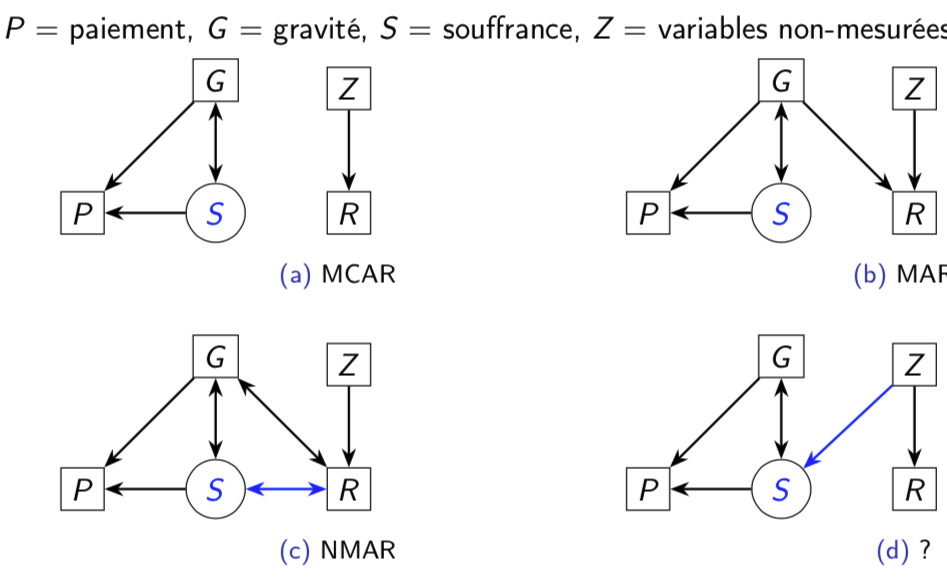
\includegraphics[scale=0.2]{src/ACT-3114/data-schema-missing.png}

Pour exemple, si on cherchait à supprimer des valeurs d'une BD:
\begin{description}
	\item[MCAR]	supprime des valeurs aléatoirement;
	\item[MAR]	supprime 60\% des valeurs pour les femmes et 40 \% des valeurs pour les hommes;
	\item[NMAR]	plus il y a de sinistres observés, plus il y a de chances que les valeurs soient manquantes.
\end{description}

Ordre de restriction des différents patrons
\begin{enumerate}[leftmargin = *]
	\item	MCAR: plus \og restrictif \fg{}, car les données doivent être manquantes complètement aléatoirement;
	\item[]	Même idée que l'hypothèse de normalité est restrictive puisque les données \textit{doivent} l'être, \textbf{mais} cela nous permet d'utiliser plein de tests;
	\item[]	Comme une Bernoulli, il n'y a pas de paramètres;
	\item[]	plus restrictif alias moins flexible.
	\item	MAR: inclue les variables observées et donc il y a plus de paramètres;
	\item	NMAR: inclue toutes les variables et est donc le patron le plus flexible (alias, le moins restrictif).
\end{enumerate}

\subsection*{Visualisation et détection}
\begin{algo}{Traiter les données manquantes}
\begin{enumerate}[leftmargin = *]
	\item	Détectez, visualisez et documentez les données manquantes;
	\item	Identifier le patron de non-réponse;
	\item[]	Pour exemple, voici quelques patrons de non-réponse pour quelques variables:

	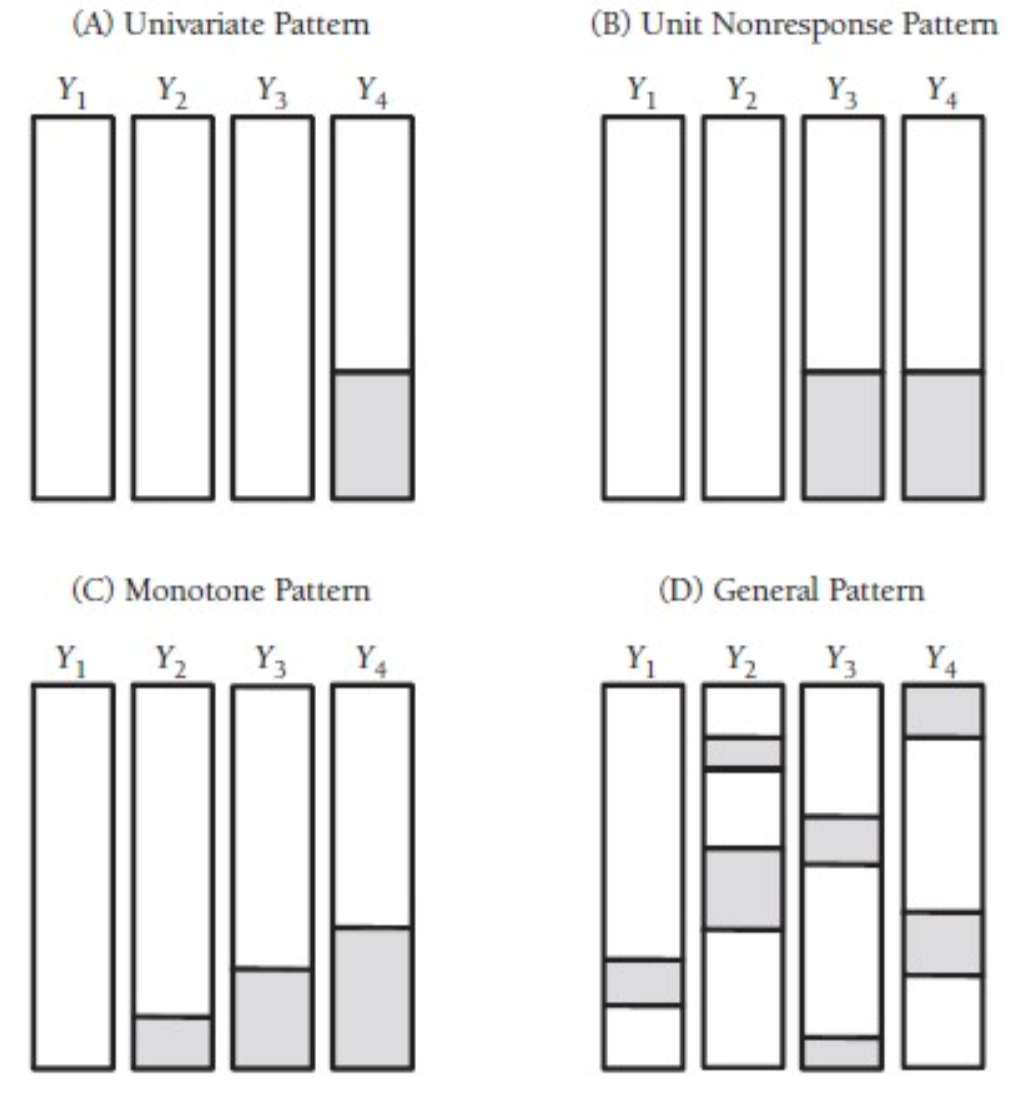
\includegraphics[scale=0.3]{src/ACT-3114/patrons-non-repoonse-exemples.png}
	\item[]	Exemple de patron univarié: concessionnaire ne pose jamais à ses assurés s'ils ont une piscine et donc la variable est manquante dans toutes ses données;
	\item	Comparer les distributions des autres variables selon la valeur des variables indicatrices $R_{1j}, \dots, R_{nj}$;
\end{enumerate}
\end{algo}

\subsection*{Identification des types de non-réponses}
\begin{itemize}[leftmargin = *]
	\item	Pour les variables continues, on fait un \textbf{test $t$ sur les différences de moyenne} au lieu du khi-carré de Pearson comme pour MCAR;
	\item	Problème de comparaisons multiples;
	\item	Le test MCAR de Little est peu utile, mais peut adresser le problème de comparaisons multiple avec une hypothèse testant toutes les variables;
\end{itemize}

\subsection*{Traitement des données manquantes}

En continuant la mise en contexte, on suppose qu'on veut estimer le vecteur $\matr{\beta}$ des coefficients de la régression logistique pour prédire la probabilité de paiement;
Une question valide est si les options pour le traitement des données manquantes dépendent du \textbf{type} de non-réponse

\textbf{Options} de traitement:
\begin{enumerate}[leftmargin = *]
	\item	Utiliser seulement les \textbf{cas complets} \textit{(complete-case analysis)};
		\begin{itemize}[leftmargin = *]
		\item	L'option par défaut pour les fonctions :
			\begin{center}
			\texttt{lm, glm, na.rm, na.omit}
			\end{center}
		\item	\textbf{Impact}:
			\begin{itemize}[leftmargin = *]
			\item[$\color{red}\downarrow$]	taille de l'échantillon	\\
			\item[$\color{red}\downarrow$]	taille de la corrélation des variables	\\
			\item[$\color{blue}\uparrow$]	variance des estimateurs	\\
			\item[$\color{red}\downarrow$]	puissance des tests	\\
			\end{itemize}
		\item	Uniquement valide sous \textcolor{ao(english)}{MCAR};
		\end{itemize}
	\item	Utiliser seulement les \textbf{cas disponibles} \textit{(available-case analysis)};
		\begin{itemize}[leftmargin = *]
		\item	Utilise uniquement les données observées pour l'analyse;
		\item	Rarement applicable;
		\item	$\color{red}\downarrow$ la taille de l'échantillon \textbf{moins} qu'en utilisant d'uniquement les cas complets;
		\item	\textcolor{ao(english)}{Sans biais} \textbf{uniquement} sous \textcolor{ao(english)}{MCAR};
		\end{itemize}
	\item	\textbf{Imputation} simple par la \textbf{moyenne ou} la \textbf{médiane}
		\begin{itemize}[leftmargin = *]
		\item	Substitue les \texttt{NA} par la moyenne ou médiane de la variable;
		\item	\textbf{Impact}:
			\begin{itemize}[leftmargin = *]
			\item[$\color{red}\downarrow$]	variabilité de la variable	\\
			\item[$\color{red}\downarrow$]	corrélation de la variable avec les autres	\\
			\end{itemize}
		\item	Même sous MCAR, les données sont \textbf{sévèrement} \og distorted \fg{};
		\end{itemize}
	\item	Imputation simple par une régression;
		\begin{itemize}[leftmargin = *]
		\item	Substitue les \texttt{NA} par la prévision d'une régression de la variable sur les autres avec les cas complets;
		\item	Si plusieurs variables ont des données manquantes, leurs patrons doivent être traités séparément;
		\item	L'inter \textbf{corrélation} des variables est \textbf{conservée}, mais est \textcolor{blue}{\textbf{surestimée}} (même si MCAR);
		\item	La variance est \textcolor{red}{\textbf{sous-estimée}}, mais \textbf{moins} qu'avec l'imputation par la moyenne;
%%%	-------------------------------
%%%	NOTE:
%%%	+	See if I can change the format for this to be arrows like the rest once 
%%%		I have a better understanding of whether I should make a distinction 
%%%		between "sous-estimé" and "diminution";
%%%	-------------------------------
		\end{itemize}
	\item	Imputation stochastique par une régression;
		\begin{itemize}[leftmargin = *]
		\item	Ajoute un terme d'erreur $\varepsilon$ (normalement distribué) à la prévision de la régression;
%%%	-------------------------------
%%%	NOTE:
%%%	+	Je ne comprends pas ce que ça veut dire "dans un patron";
%%%	+	Pensais que patron c'était une pattern alors comment plusieurs variables pourraient être manquantes dans un patron?
%%%	-------------------------------
		\item	\textit{Si plusieurs variables sont manquantes dans un patron, les erreurs sont corrélées}
		\item	Corrige les biais pour la méthode d'imputation par la régression (sous-estimation de la variance et surestimation de l'inter corrélation des variables);
%%%	-------------------------------
%%%	NOTE:
%%%	+	Je ne comprends pas ce qu'on veut dire par "dans les calculs";
%%%	+	En tenir compte implique faire quoi?
%%%	+	Faire un ajustement en calculant le biais?
%%%	-------------------------------
		\item	La variance des paramètres est \textcolor{red}{\textbf{sous-estimée}}, \textit{sauf si on en tient compte dans les calculs};
		\item	Fonctions \texttt{R} utiles du paquetage \texttt{mice}:
			\begin{center}
			\texttt{mice.impute.norm.nob(), mice.impute.norm()}
			\end{center}
		\end{itemize}
	\item	Imputation simple \textit{hot-deck};
		\begin{itemize}[leftmargin = *]
		\item	Substitue les valeurs \texttt{NA} d'une observation par les valeurs observées d'une autre observation choisie aléatoirement;;
		\item	Habituellement, cette observation fait parmi d'un sous-ensemble d'observations \textit{proches} (pensez au $K$-NN, clustering, etc.);
		\item	Souvent utilisée pour les sondages;
%%%	-------------------------------
%%%	NOTE:
%%%	+	Pourquoi ça ne les altère pas?
%%%	+	Puisqu'il aurait seulement le patron par observation et donc elle ne serait aucunement reliée à une autre observation?
%%%	-------------------------------
		\item	N'altère par les distributions univariées
		\item	$\color{red}\downarrow$	l'inter corrélation des variables;
		\item	Biais des estimations des coefficients $\matr{\beta}$ de régression;
		\end{itemize}
	\item	Imputation \textbf{multiple};
		\begin{itemize}[leftmargin = *]
		\item	Répète l'imputation stochastique et agrège les résultats;
%%%	-------------------------------
%%%	NOTE:
%%%	+	Est-ce que "non biaisée" est vraiment équivalent à "estime correctement"?
%%%	+	Je pose que oui;
%%%	-------------------------------
		\item	Ce faisant, la variabilité additionnelle dût à l'imputation des valeurs manquante est adressée et la variance des estimateurs est \textit{non biaisée};
		\end{itemize}
\end{enumerate}

Autres méthodes:
\begin{itemize}[leftmargin = *]
	\item	MLE avec données manquantes;
	\item	Algorithme EM (expectation-maximisation)
	\item	Inférence bayésienne;
\end{itemize}

\subsection*{Conseils}
\begin{itemize}[leftmargin = *]
	\item	Conserver un script pour le traitement de données manquantes et ne \textbf{pas hard-coder};
	\item	\textit{Utiliser une méthode d'imputation qui respecte le format de la variable;}
	\item	Plus la proportion de non-réponses est élevée, plus l'impact sur l'analyse sera important;
	\item	S'il y a plusieurs patrons de non-réponse différents, l'ordre dans lequel les données sont imputées est important;
\end{itemize}

\newpage

\section{Analyse en composantes principales}

\begin{definitionNOHFILLsub}[Fonctions \texttt{R}]
\texttt{PCA(X = , scale = T)}
\begin{itemize}
	\item	On donne la BD en premier argument et standardise avec le deuxième.
\end{itemize}
\end{definitionNOHFILLsub}

\newpage

\section{Apprentissage non supervisée}

\begin{definitionNOHFILLsub}[Liaisons]
\begin{description}
	\item[Complete linkage]	Mesure la distance maximale (les deux points les plus éloignés) des groupes et on choisit la plus petite distance.
	\item[Single linkage]	Mesure la distance minimale (les deux points les plus proches) des groupes et on choisit la plus petite distance.
	\item[Average linkage]	Mesure la moyenne des distances entre les points de chacun des groupes puis on choisit la plus petite distance.
	\item[Centroid linkage]	Assigne un centroïd à chaque groupe ayant comme coordonnées la moyenne des observations du groupe.
	\item[Ward]	La distance correspond à l'augmentation de l'EQM suite à la fusion d'un groupe. L'EQM commence à zéro puisque chaque observation à son propre groupe. Ceci est utile lorsque l'on croit que l'EQM devrait être petite.
\end{description}
\end{definitionNOHFILLsub}

\subsection*{Concepts de distance et similarité}

\begin{definitionNOHFILL}[Classification]
\begin{description}
	\item[supervisée]	Lorsqu'on connaît les \textbf{étiquettes} des groupes et on veut prédire l'appartenance à un groupe pour de nouvelles observations;
		\begin{itemize}[leftmargin = *] 
		\item	\og \textit{Classification} \fg{}.
		\end{itemize}
	\item[non supervisée]	Lorsqu'on ne sait pas combien de groupes il y a ni comment qu'ils sont formés;
		\begin{itemize}[leftmargin = *]
		\item	Alias partitionnement ou regroupement;
		\item	\og \textit{Clustering} \fg{}.
		\end{itemize}
\end{description}
\end{definitionNOHFILL}

\begin{conceptgen}{Conditions des mesures de distance}
Une mesure de distance dans l'espace $\mathbb{E}$ est une application $d : E \times E \rightarrow \mathbb{R}^{+}$ respectant ces 3 conditions:
\begin{enumerate}[leftmargin = *]
	\item	Symétrique\\
	$d(i, j) = d(j, i), \, \forall i, j \in E$;
	\item	Nulle pour un même objet\\
	$d(i, j) = 0 \Leftrightarrow i = j, \, \forall i, j \in E$;
	\item	Satisfait l'inégalité du triangle\\
	$d(i, k) \le d(i, j) + d(j, k), \, \forall i, j, k \in E$.
\end{enumerate}
\end{conceptgen}

\begin{definitionNOHFILL}[Distance de Minkowski $\ell_{q}$]
Soit 2 points $(x_{11}, \dots, x_{1d})$ et $(x_{21}, \dots, x_{2d})$ dans l'espace $\mathbb{R}^{d}$.

Alors, pour $q \ge 1$:
\begin{align*}
	\ell_{q}
	&=	\Vert \matr{x_{1} - x_{2}} \Vert_{q}	\\
	&=	\left( \sum_{i = 1}^{d} |x_{1i} - x_{2i}|^{q} \right)^{1/q}	\\
\end{align*}

Deux cas particuliers sont bien connus:
\begin{itemize}[leftmargin = *]
	\item	$q = 1$:	Distance de Manhattan $\ell_{1}$;
	\item	$q = 2$:	Distance euclidienne $\ell_{2}$.
\end{itemize}

\tcbline

La version standardisée de la distance euclidienne se simplifie à:
\begin{align*}
	d(\matr{x_{1}, x_{2}})
	&=	\sqrt{\sum_{i = 1}^{d} \left( \frac{x_{1i} - x_{2i}}{s_{i}} \right)^{2}}
\end{align*}
\end{definitionNOHFILL}

\begin{conceptgen}{Conditions des indices de similarité}
Une mesure de similarité entre 2 objets dans l'espace $\mathbb{E}$ est une application $s : E \times E \rightarrow [0, 1]$ respectant ces 2 conditions:
\begin{enumerate}[leftmargin = *]
	\item	Symétrique\\
	$s(i, j) = s(j, i), \, \forall i, j \in E$;
	\item	Un même objet est identique et maximise la similarité\\
	$s(i, j) = 1 \ge s(i, j), \, \forall i, j \in E$.
\end{enumerate}

\tcbline

De plus, l'indice de similarité peut être obtenu d'une mesure de distance $s(i, j) = \frac{1}{1 + d(i, j)}$.\\
Également, on peut définir un indice de \textbf{dissimilarité} avec $\tilde{d}(i, j) = 1 - s(i, j)$.
\end{conceptgen}

\begin{conceptgen}{Types de variables binaires}
\begin{description}
	\item[symétrique]	Si une variable binaire est \textbf{symétrique}, c'est que ses deux niveaux sont aussi fréquents;
		\begin{itemize}[leftmargin = *]
		\item	Par exemple, qu'une personne soit un homme ou une femme.
		\end{itemize}
	\item[asymétrique]	Si une variable binaire est \textbf{asymétrique}, c'est qu'un niveau est plus rare que l'autre.
		\begin{itemize}[leftmargin = *]
		\item	On dénote le niveau plus rare par 1;
		\item	Par exemple, deux personnes ayant brisé leur orteil sont plus semblables que deux personnes ayant un mal de tête.
		\end{itemize}
\end{description}
\end{conceptgen}

\begin{conceptgen}{Mesures de similarité (variables binaires ou ordinales)}
\begin{center}
	Variable binaire symétrique
\end{center}
La \textbf{proportion d'accord} (\og \textit{simple matching coefficient} \fg{}):
\begin{align*}
	s(\matr{x_{1} - x_{2}})
	&=	\frac{1}{d}	\sum_{i = 1}^{d} \bm{1}_{\{x_{1i} = x_{2i}\}}
\end{align*}
\tcbline
\begin{center}
	Variable binaire asymétrique
\end{center}
\textbf{L'indice de Jaccard}:
\begin{align*}
	s(\matr{x_{1} - x_{2}})
	&=	\frac{\sum_{i = 1}^{d} x_{1i}x_{2i}}{\sum_{i = 1}^{d} \{1 - (1 - x_{1i})(1 - x_{2i})\}}
\end{align*}
\tcbline
\begin{center}
	Variable binaire asymétrique
\end{center}
On assigne un score numérique (positif) à chaque niveau et traite la variable comme une variable numérique.
\end{conceptgen}

\begin{conceptgen}{Similarité de Gower}
Dans le cas où les variables sont de plusieurs types:
\setlength{\mathindent}{-1cm}

\begin{align*}
	G(\matr{x_{1} - x_{2}})
	&=	\frac{\sum_{i = 1}^{d} w_{i} \gamma_{i} (x_{1i}, x_{2i}) s_{i}(x_{1i}, x_{2i})}{\sum_{i = 1}^{d} w_{i} \gamma_{i} (x_{1i}, x_{2i})}
\end{align*}
\setlength{\mathindent}{1cm}
où le poids des variables $w_{i} > 0$.

Également, avec l'étendu dénoté $r_{i} = \max(x_{1i}, \dots, x_{ni}) - \min(x_{1i}, \dots, x_{ni})$, si $\matr{x_{i}}$ est :

\begin{itemize}[leftmargin = *]
	\item	numérique ou ordinale, $\gamma_{i} (x_{1i}, x_{2i}) = 1$ et  $s_{i}(x_{1i}, x_{2i}) = 1 - \frac{|x_{1i} - x_{2i}|}{r_{i}}$;
	\item	binaire symétrique, $\gamma_{i} (x_{1i}, x_{2i}) = 1$ et  $s_{i}(x_{1i}, x_{2i}) = 1_{\{x_{1i} = x_{2i}\}}$;
	\item	binaire asymétrique, $\gamma_{i} (x_{1i}, x_{2i}) = 1 - (1 - x_{1i})(1 - x_{2i})$ et  $s_{i}(x_{1i}, x_{2i}) = 1_{\{x_{1i} = x_{2i}\}}$.
\end{itemize}
\end{conceptgen}

\begin{conceptgen}{Similarité du Cosinus}
Un exemple d'application de la similarité du Cosinus est l'analyse de texte. On assigne une variable indicatrice pour chaque mot selon s'il est présent ou non (il y a donc \textit{beaucoup} de colonnes). Par la suite, on assigne un poids $w_i$ à chaque variable selon son importance. Donc, par exemple, la mesure peut calculer la similarité entre deux textes.

\begin{align*}
	s_{i}(x_{1i}, x_{2i}) 
	&=	\frac{\sum_{i = 1}^{d} w_{i} x_{1i} x_{2i}}{\sqrt{\sum_{i = 1}^{d}w_{i}x_{1i}^{2}\sum_{i = 1}^{d} w_{i} x_{2i}^{2}}}
\end{align*}
\end{conceptgen}

%\columnbreak

\subsection*{$K$-means clustering}
\begin{distributions}[Notation]
\begin{itemize}[leftmargin = *]
	\item	Soit les observations $\matr{x_{1}, \dots, x_{n}}$ formées de variables \textbf{quantitatives};
	\item	Soit les sous-ensembles $C_{1}, \dots, C_{k}$;
	\item	Chaque observation appartient seulement à un groupe et donc les ensembles sont \textbf{mutuellement exclusifs}
		\begin{align*}
		C_{j} \cap C_{j'} = \emptyset, \, \forall j \neq j', j, \, j' \in \{1, \dots, k\}
		\end{align*}
\end{itemize}
\end{distributions}

\subsection*{Hierarchical clustering}

\begin{definitionNOHFILLsub}[Fonctions \texttt{R}]
\texttt{hclust(d = dist(data), method = "complete")}.
\begin{itemize}
	\item	On spécifie la méthode de liaison avec \texttt{method = };
	\item	On donne en argument une matrice de distance pour \texttt{d = }.
\end{itemize}

On peut élaguer avec \texttt{cutree(tree = , k = , h = ))}.
\begin{itemize}
	\item	On donne en premier argument le dendrogramme;
	\item	On peut soit spécifier un nombre de groupes avec \texttt{k = } ou une hauteur avec \texttt{h = }.
\end{itemize}
\end{definitionNOHFILLsub}

\subsection*{Paramètres}
Un paramètre est appris par l'entraînement.\\
Un hyperparamètre informe l'entraînement comme tel et est fixé à l'avance. \\
Par exemple, $k$ est un hyperparamètre dans le $K$-NN, et c'est le seul.

\subsection*{Échantillonage}
Pour atténuer le problème de débalancement:
\begin{description}
	\item[sur-échantillonnage]	dupliquer au hasard des observations sous observées.
	\item[sous-échantillonnage]	ignorer une partie des observations ayant l'étiquette plus fréquemment rencontrée.
\end{description}
D'une manière ou l'autre, le jeu de données étudié est alors plus balancé.

\pagebreak

\section{Apprentissage supervisé}
\begin{definitionNOHFILL}[Inférence]
Comprendre le lien entre les prédicteurs et la \textit{variable réponse}. Par exemple, tests d'hypothèses, intervalles de confiance et interprétations.\\

De façon générale, on préfère des modèles moins flexible puisqu'ils sont plus interprétables pour  faire de l'inférence.
\end{definitionNOHFILL}

\begin{definitionNOHFILL}[Prévisions]
Prédire le plus précisément possible la valeur de $Y$ étant donné les valeurs des covariables.\\

Si $\hat{f}$ peut estimer $f$, une prévision pour la variable d'intérêt $Y$ étant donné les valeurs de $x_{1}, \dots, x_{p}$ est $\hat{Y} = \hat{f}(x_{1}, \dots, x_{p})$. \\

Il y a deux types de techniques qui servent à estimer $f$:
\begin{enumerate}
	\item	L'apprentissage automatique et
	\item	La modélisation statistique.
\end{enumerate}
\end{definitionNOHFILL}


\begin{definitionNOHFILLsub}[Apprentissage automatique]
\begin{description}
	\item[But principal]	Prédire la valeur de $Y$;
	\item[$Y$]	On ne cherche pas à explicitement estimer ni interpréter l'effet de la valeur des variables $x_{j}$ sur $Y$;
	\item[Fluctuation aléatoire]	N'est \textbf{pas} un intérêt majeur;
	\item[hypothèses à priori sur $f$]	Peu d'hypothèses à priori, on se base sur les données.
\end{description}
\end{definitionNOHFILLsub}

\begin{definitionNOHFILLsub}[Modélisation statistique]
\begin{description}
	\item[But principal]	Estimer explicitement et interpréter l'effet de la valeur des variables $x_{j}$ sur $Y$;
	\item[$Y$]	Peut prédire $Y$ avec le modèle;
	\item[Fluctuation aléatoire]	Est un intérêt puisqu'on veut parfois simuler de nouvelles observations de $Y$;
	\item[hypothèses à priori sur $f$]	Sont requises afin d'estimer seulement ce qui est inconnu de $f$ (c.-à-d., les paramètres).
\end{description}
\end{definitionNOHFILLsub}

Flexible vs inflexible:
\begin{itemize}
	\item	With alot of data and few predictors, a flexible approach would perform better. The amount of data permits us to fit more accurate predictors and the variance is limited by the number off parameters. 
	\item	With a small number of observations and many predictors, an inflexible approach would perform better. The small number of observations leads to worse parameter estimates and the combined large number of predictors leads to the possiblity of overfitting.
	\item	A flexible approach would fit better when there is a non-linear relationship between the predictors and the response variable. An inflexible is more restrained and can't capture it.
	\item	A flexible approach would fit worse when there is high variance amongst the error terms. The flexible model would try to fit this error and drastically increase variance.
\end{itemize}


\begin{center}
	\textbf{Décomposition Biais-Variance}\\
\tikzset{every picture/.style={line width=0.75pt}} %set default line width to 0.75pt        

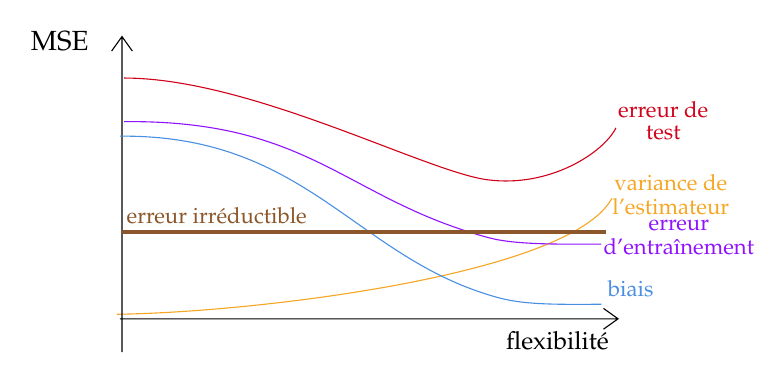
\begin{tikzpicture}[x=0.75pt,y=0.75pt,yscale=-1,xscale=1]
%uncomment if require: \path (0,300); %set diagram left start at 0, and has height of 300

%Curve Lines [id:da5387525772336879] 
\draw [color={rgb, 255:red, 245; green, 166; blue, 35 }  ,draw opacity=1 ]   (96.72,145.8) .. controls (162.17,145) and (315.17,127) .. (335.17,90) ;
%Shape: Axis 2D [id:dp3627700228658668] 
\draw  (98.17,148) -- (338.17,148)(99.17,12) -- (99.17,164) (331.17,143) -- (338.17,148) -- (331.17,153) (94.17,19) -- (99.17,12) -- (104.17,19)  ;
%Curve Lines [id:da8647605952322346] 
\draw [color={rgb, 255:red, 74; green, 144; blue, 226 }  ,draw opacity=1 ]   (98.17,60) .. controls (188.81,59.16) and (211.71,119.46) .. (281.17,138) .. controls (294.46,141.55) and (312.97,141) .. (330.17,141) ;
%Curve Lines [id:da4811730718241043] 
\draw [color={rgb, 255:red, 144; green, 19; blue, 254 }  ,draw opacity=1 ]   (100.17,53) .. controls (190.81,52.16) and (206.71,90.46) .. (276.17,109) .. controls (289.46,112.55) and (312.97,112) .. (330.17,112) ;
%Curve Lines [id:da8073024446675301] 
\draw [color={rgb, 255:red, 208; green, 2; blue, 27 }  ,draw opacity=1 ]   (100.17,32) .. controls (161.17,32) and (245.17,77) .. (275.17,81) .. controls (305.17,85) and (331.17,68) .. (337.17,56) ;
%Straight Lines [id:da4343589431923036] 
\draw [color={rgb, 255:red, 139; green, 87; blue, 42 }  ,draw opacity=1 ][line width=1.5]    (99.17,106) -- (332.17,106) ;

% Text Node
\draw (283,153) node [anchor=north west][inner sep=0.75pt]   [align=left] {{\small flexibilité}};
% Text Node
\draw (54,8) node [anchor=north west][inner sep=0.75pt]   [align=left] {MSE};
% Text Node
\draw (332,128) node [anchor=north west][inner sep=0.75pt]   [align=left] {{\footnotesize \textcolor[rgb]{0.29,0.56,0.89}{biais}}};
% Text Node
\draw (330,99) node [anchor=north west][inner sep=0.75pt]  [color={rgb, 255:red, 144; green, 19; blue, 254 }  ,opacity=1 ] [align=left] {{\footnotesize \shortstack{erreur\\ d'entraînement}}};
% Text Node
\draw (334.17,77) node [anchor=north west][inner sep=0.75pt]  [color={rgb, 255:red, 144; green, 19; blue, 254 }  ,opacity=1 ] [align=left] {\textcolor[rgb]{0.96,0.65,0.14}{{\footnotesize \shortstack{variance de\\ l'estimateur}}}};
% Text Node
\draw (337,42) node [anchor=north west][inner sep=0.75pt]  [color={rgb, 255:red, 144; green, 19; blue, 254 }  ,opacity=1 ] [align=left] {{\footnotesize \textcolor[rgb]{0.82,0.01,0.11}{\shortstack{erreur de\\ test}}}};
% Text Node
\draw (100.17,93) node [anchor=north west][inner sep=0.75pt]  [font=\footnotesize,color={rgb, 255:red, 139; green, 87; blue, 42 }  ,opacity=1 ] [align=left] {erreur irréductible};
\end{tikzpicture}
\end{center}

\pagebreak

\section{Arbres de classification et de régression}

\begin{description}
	\item[CART]	Classification and Regression Tree.
\end{description}

\begin{center}
	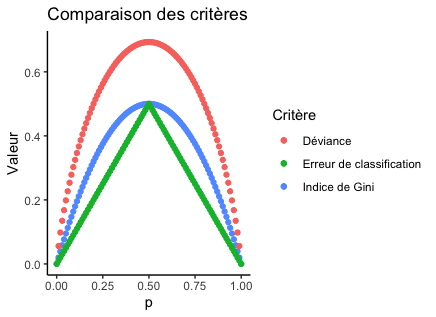
\includegraphics[scale=0.4]{src/ACT-3114/CART-criteria.png}
\end{center}

\begin{definitionNOHFILL}[Indice de Gini]
Mesure de la variance totale entre les $K$ classes:
\begin{align*}
	G	
	&=	\underset{k = 1}{\overset{K}{\sum}} \hat{p}_{mk} (1 - \hat{p}_{mk})
\end{align*}
\begin{itemize}[leftmargin = *]
	\item	L'indice de Gini mesure la \textbf{pureté des nœuds}, si les proportions échantillonnales sont près de 0 ou 1, $G$ sera très petit.
	\item	C'est la mesure par défaut avec la fonction pour une classification \texttt{rpart(method = "class")}.
\end{itemize}
\end{definitionNOHFILL}

\begin{definitionNOHFILL}[Déviance, ou entropie croisée]

\begin{align*}
D	
	&=	-\underset{k = 1}{\overset{K}{\sum}} \hat{p}_{mk} \log(\hat{p}_{mk})
\end{align*}
%\begin{itemize}[leftmargin = *]
%	\item	
%\end{itemize}
\end{definitionNOHFILL}

\begin{definitionNOHFILL}[Élagage par coût-complexité]
\begin{description}
	\item[cp]	Paramètre de complexité.
	\item[|T|]	Nombre de feuilles (\og \textit{terminal nodes} \fg{}).
	\item[Critère de coût-complexité]
\end{description}
\begin{align*}
	C_{cp}(T)	
	&=	\underset{m = 1}{\overset{| T |}{\sum}}\underset{i:\bm{x}_{i} \in R_{m}}{\sum} (y_{i} - \hat{y}_{R_{m}})^{2} + cp | T |
\end{align*}
\begin{itemize}[leftmargin = *]
	\item	Le critère permet d'ajuster le modèle en balancant la \textbf{complexité} de l'arbre \textbf{\textit{et}} la \textbf{qualité} de l'ajustement.
\end{itemize}
\end{definitionNOHFILL}

Le seul point négatif des CART est leur précision qui a tendance à être mauvaise.

\paragraph{Note}	Le point de séparation doit être un qui parmi l'ensemble donné. Par exemple, pour $\{1, 3\}$  on ne peut pas stipuler un point de séparation à 2.

\begin{definitionNOHFILLsub}[Fonction \texttt{R}]
Paquetage \texttt{rpart} (Recursive Partioning And Regression Trees) dont la fonction \texttt{rpart()}.
\begin{itemize}
	\item	On utilise \texttt{weights = } si on veut pondérer des observations.
	\item	On utilise \texttt{cost = } pour spécifier un vecteur de coûts associés à chaque variable dans la séparation des données. \\
			Cela peut s'avérer utile pour pénaliser une variable qu'on voudrait idéalement utiliser seulement si son pouvoir prédictif est très grand.
	\item	\texttt{method = } permet de spécifier si l'arbre doit retourner une réponse de type "class" ou "numeric".
	\item	\texttt{control = list(maxdepth = )} permet de spécifier la profondeur de l'arbre $d$.
\end{itemize}
%%	voir labo sur apprentissage supervisé pour exemple avec CARET
%%	confusionMatrix() pour un tableau de confusion avec les statistiques en plus

Élagage: \texttt{cv.tree(tree, FUN = )}
\begin{itemize}
	\item	Pour un arbre de régression, on utilise \texttt{FUN = prune.tree};
	\item	Pour un arbre de classification, on utilise \texttt{FUN = prune.misclass}.
\end{itemize}
\end{definitionNOHFILLsub}

\newpage

\section{Bagging et forêts aléatoires}
En raison du nombre faible d'observations dans plusieurs des nœuds:
\begin{itemize}[leftmargin = *]
	\item	La variance des prévisions est très élevée.
	\item	L'arbre n'est pas robuste---des différents échantillons mènent à des points de séparation différents et donc des prévisions différentes.
\end{itemize}

Pour aider à atténuer ce problème, nous voyons deux \textbf{méthodes d'ensemble}.
\begin{definitionNOHFILL}[Méthode d'ensemble]
Algorithme de prévision qui agrège les prévisions de plusieurs modèles différents.

\begin{itemize}[leftmargin = *]
\item	Cela est particulièrement utile si les modèles ont une \textbf{grande variance} et donc est rarement utilisé avec des GLMs.
\end{itemize}
\end{definitionNOHFILL}

\begin{definitionNOHFILLsub}[Bagging]
Méthode d'ensemble générale qui permet de réduire la variance d'un modèle d'apprentissage statistique.
\begin{itemize}[leftmargin = *]
	\item	Bien que le bagging peut être appliqué à n'importe quel modèle, on le voit uniquement dans le contexte d'arbres;
	\item	Prendre la moyenne des prévision obtenues avec différents échantillons d'entrainement permet de réduire la variance des prévisions;
	\item	Il s'ensuit que les prévisions sont améliorées: 
	\setlength{\mathindent}{-1.5cm}
		\begin{align*}
		\text{E}\left[\shortstack{erreur quadratique\\ de prévision}\right]
		&=	biais^{2} + \text{variance} + \varepsilon
		\end{align*}
	\setlength{\mathindent}{1cm}
\end{itemize}
\end{definitionNOHFILLsub}

\begin{algo2}[Algorithme de bagging sur les arbres]
Pour $b = 1, 2, \dots, B$,
\begin{enumerate}
	\item	Générer un \textbf{échantillon bootstrap} $\mathcal{D}^{b}$ de l'échantillon d'entrainement;
		\begin{itemize}[leftmargin = *]
		\item	L'échantillon est de la même taille que l'échantillon d'entrainement initial.
		\end{itemize}
	\item	Ajuster un (gros) arbre de régression sur $\mathcal{D}^{b}$ pour obtenir la prévision $f^{b}(\bm{x})$.
		\begin{itemize}[leftmargin = *]
		\item	Il n'y a pas d'élagage avec $cp = 0$;
		\item	Les arbres ont une grande variance et un faible biais;
		\item	La taille de l'arbre est contrôlée avec \texttt{maxdepth} (nombre maximal de niveaux) et \texttt{minbucket} (taille minimale d'un nœud).
		\end{itemize}
		\begin{align*}
		f_{\text{bag}}(\bm{x})
		&=	\frac{1}{B} \sumz{B}{b = 1} f^{b}(\bm{x})
		\end{align*}
\end{enumerate}

\paragraph{Note}	Le nombre d'arbres $B$ doit être assez gros (100, 1 000, etc.) et \textbf{une grande valeur ne mène pas à un sur ajustement} \textit{habituellement}; c'est les autres paramètres qui vont contrôler le sur ajustement.
\end{algo2}

\subsubsection*{Prévision}
\begin{itemize}[leftmargin = *]
	\item	La probabilité de ne pas piger une observation parmi $n$, avec remise, est $1 - \frac{1}{n}$.\\
			La probabilité qu'elle ne soit pas dans l'échantillon de taille $n$ du tout est $(1 - \frac{1}{n})^{n}$.\\
			Lorsque $n \rightarrow \infty$, $\limz{n}{\infty}(1 - \frac{1}{n})^{n} = \textrm{e}^{-1} = 36.79\% \approx 1/3$.\\
			On dit donc que, en moyenne, chaque arbre dans le bagging n'utilise pas environ 1/3 des données;
	\item	Les observations qui ne sont pas utilisées sont les observations dites "Out-Of-Bag" (OOB);
	\item	Pour chaque itération du bagging, on calcule la prévision pour les observations OOB.\\
			Pour chaque observation $i$, on calcule la moyenne des prévision pour en obtenir une seule;
	\item	L'EQM des ces prévisions calculée à la fin est \textbf{l'erreur OOB}.\\
			Lorsque $B$ est suffisamment grand, elle se stabilise pour être équivalente à l'erreur obtenue avec LOOCV.
\end{itemize}

Limitations
\begin{itemize}
	\item[$\color{blue}+$]	Les prévisions sont beaucoup plus "lisses" (voir p. 24);
	\item[$\color{red}-$]	Les prévisions sont beaucoup moins interprétables.
		\begin{itemize}[leftmargin = *]
		\item	Notamment, avec plus de 2 variables, on ne peut pas visualiser les prévisions et donc on ne peut pas comprendre pourquoi l'algorithme fait ses décisions.
		\end{itemize}
\end{itemize}

\begin{definitionNOHFILLsub}[Forêts aléatoires]
Méthode d'ensemble qui s'inspire du bagging mais qui permet de \textbf{décorréler les arbres} en:
\begin{itemize}[leftmargin = *]
	\item	On choisit un échantillon bootstrap d'une plus petite taille \texttt{sampsize}, par exemple 	50\% ou 75\% de la taille de l'échantillon d'entrainement;
		\begin{itemize}[leftmargin = *]
		\item	On note que logiquement le plus il y a de prédicteurs alors le plus les arbres seront corrélés entre eux (voir p. 31 des NDC).
		\end{itemize}
	\item	À chacun des nœuds de chacune des itérations dans la construction de l'arbre, on choisit aléatoirement $m$ prédicteurs à considérer pour la séparation.
		\begin{itemize}[leftmargin = *]
		\item	La valeur de $m \in \{1, \dots, d\}$ est un hyperparamètre mais on choisit souvent $m \approx \lfloor d / 3\rfloor$ en régression et $m \approx \sqrt{d}$ en classification.
		\end{itemize}
\end{itemize}

Les améliorations apportées par la forêt sont plus utiles lorsqu'ils y a beaucoup de prédicteurs corrélés dans les données. La corrélation sera encore plus importante s'il y a certaines variables qui très importantes puisque tous les arbres vont l'avoir ce qui augmente la corrélation.

\end{definitionNOHFILLsub}

\subsubsection*{Mesure de l'importance des variables}

\begin{description}
	\item[Permutation]	On substitue aléatoirement la variable $j$ pour une observation et effectue une prévision avec cette substitution qui n'a aucun rapport avec le restant de la ligne.
		\begin{itemize}[leftmargin = *]
		\item	Si la nouvelle prévision est mauvaise alors la variable est importante, et vice-versa;
		\item	En \texttt{R} cette méthode s'appelle \og \textit{mean decrease in accuracy} \fg{}.
		\end{itemize}
	\item[Diminution totale]	dans la fonction de perte due à une séparation sur la variable $j$, et on compare pour $j = 1, 2, \dots, d$.
		\begin{itemize}[leftmargin = *]
		\item	Pour chaque séparation qui a lieu sur la variable $j$, je vais calculer la diminution de la fonction de perte (donc à tous les nœuds de tous les arbres);
		\item	Souvent on divise par la valeur maximale pour avoir des importances entre 0 et 1;
		\item	En \texttt{R} cette méthode s'appelle \og \textit{mean decrease in node impurity} \fg{}.
		\end{itemize}
\end{description}
On peut les visualiser en \texttt{R} avec \texttt{varImpPlot}.

La mise en garde des arbres est que le modèle est beaucoup moins interprétable et beaucoup plus lourd à calculer.

\newpage

\section{Boosting et Gradient Boosting}

\begin{distributions}[Terminologie]
\begin{description}
	\item[$\lambda$]	Taux d'apprentissage (alias, le paramètre de régularisation).
\end{description}
		\begin{itemize}[leftmargin = *]
		\item	Le diminuer mène toujours à une meilleur performance, au prix d'un plus grand nombre d'arbres $T$.
		\item	En pratique, on choisit la plus petite valeur de $\lambda$ qui permet un temps de calcul raissonable.
		\end{itemize}
\begin{description}
	\item[$T$]	Nombre d'itérations.
\end{description}
\begin{itemize}[leftmargin = *]
	\item	Normalement assez grand mais peut mener à un surajustement.
\end{itemize}
\begin{description}
	\item[$d$]	Profondeur des arbres à chaque itération.
\end{description}
\begin{itemize}[leftmargin = *]
	\item	Souvent, $d = 1$ pour des souches ce qui mène à un modèle additif;
	\item	Plus $d$ est élevé, plus les interactions d'ordre élevé peuvent être captées mais il est rare que $d > 7$ soit utile.
\end{itemize}
\begin{description}
	\item[$\delta$]	Pourcentage de sous-échantillonnage.
\end{description}
\begin{itemize}[leftmargin = *]
	\item	Souvent 50\% ou 75\%.
\end{itemize}
\end{distributions}

\subsection*{Boosting}
Le boosting permet de combiner plusieurs modèles faibles en un prédicteur puissant.
\begin{itemize}[leftmargin = *]
	\item	À chaque itération, un arbre tente d'améliorer ce que le modèle ne prédit pas bien.
	\item	Le boosting est itératif et donc, en contraste aux forêts aléatoires, l'ajustement des arbres est impacté par l'ordre.
\end{itemize}

\begin{algo2}[Algorithme de boosting (arbres de régression)]
On initialise:

\begin{align*}
	\hat{f}_{0}(\bm{x})	&=	0	&
	&\text{et}	&
	\rho_{i, 0}	&=	y_{i}, \forall i = 1, \dots, n	\\
\end{align*}

Pour chaque itération de $t = 1, \dots, T$,
\begin{enumerate}[leftmargin  = *]
	\item	Ajuster un arbre de régression de profondeur $d$ sur les résidus $(\bm{x}, \rho_{t})$.
		\begin{itemize}[leftmargin = *]
		\item	Donc, on contrôle le nombre maximal de feuilles avec $2^{d}$ feuilles;
		\item	Par exemple, si $d = 1$ c'est une souche avec 2 feuilles;
		\item	La fonction de prévision est notée \icbox{$\hat{f}^{t}_{\text{arbre}}$}.
		\end{itemize}
	\item	Mettre à jour $\hat{f}$ en ajoutant une version rapetissée de l'arbre:
		\begin{align*}
		\hat{f}_{t}(\bm{x})	&=	\hat{f}_{t - 1}(\bm{x}) + \lambda \hat{f}^{t}_{\text{arbre}}(\bm{x})
		\end{align*}
		\begin{itemize}[leftmargin = *]
		\item	Donc on ne prend pas directement la prévision de l'arbre $\hat{f}^{t}_{\text{arbre}}$ mais plutôt une fraction de la prévision selon le taux d'apprentissage $\lambda$.
		\end{itemize}
	\item	Mettre à jour les résidus:
		\begin{align*}
		\rho_{i, t}	&=	\rho_{i, t - 1} - \lambda \hat{f}^{t}_{\text{arbre}}(\bm{x}_{i})	
		\end{align*}
\end{enumerate}

La prévision du boosting pour un arbre de régression est:
\begin{align*}
	f_{\text{boost}}(\bm{x})	
	&=	\hat{f}_{T}(\bm{x})
	=	\sumz{T}{t = 1} \lambda f_{\text{arbre}}^{t}(\bm{x})	
\end{align*}
\end{algo2}

\columnbreak

\subsection*{Adaptive Boosting (Adaboost)}
Puisque les résidus n'ont pas de sens en classification, on défini la méthode Adaboost. \\

Au lieu d'avoir un même taux d'apprentissage pour tous les arbres, chacun des arbres aura une contribution différente dans la prévision finale.

\begin{algo2}[Algorithme Adaboost (arbres de classification)]
On initialise les poids des observations :
\begin{align*}
	w_{i}	
	&=	\frac{1}{n}, \;	\forall i = 1, \dots, n	\\
\end{align*}

Pour chaque itération de $t = 1, \dots, T$,
\begin{enumerate}[leftmargin  = *]
	\item	Ajuster un arbre de classification $\hat{f}_{t}(\bm{x})$ de profondeur $d$ sur les données d'entraînement en utilisant l'indice de Gini pondéré par les poids $w_{i}$.
	\item	Calculer le taux d'erreur:
		\begin{align*}
		\text{err}_{t}	
		&=	\frac{\sumz{n}{i = 1} w_{i} \times \bm{1}_{\{ y_{i} \neq \hat{f}_{t}(\bm{x}_{i}) \}}}{\sumz{n}{i = 1} w_{i}}	\\
		&=	\frac{\shortstack{la somme des poids pour\\ les observations mal classées}}{\text{la somme totale des poids}}
		\end{align*}
	\item	Calculer la contribution de l'arbre:
		\begin{align*}
			\alpha_{t}	
			&=	\log\left(\frac{1 - \text{err}_{t}}{\text{err}_{t}}\right)
		\end{align*}
	\item	Réajuster, alias \textit{\textbf{ada}}pter, les poids $\forall i = 1, \dots, n$,
		\begin{align*}
		w_{i}
		&\leftarrow	w_{i}\, \text{exp}\left\{\alpha_{i} \bm{1}_{\{ y_{i} \neq \hat{f}_{t}(\bm{x}_{i}) \}}\right\}
		\end{align*}
\end{enumerate}

Le classificateur est:
\begin{align*}
	\hat{f}_{\text{ada}}(\bm{x})	
	&=	\text{signe}\left\{ \sumz{t = 1}{T} \alpha_{t} \hat{f}_{t} (\bm{x}) \right\}
\end{align*}
\begin{itemize}[leftmargin = *]
	\item	On traite les prévisions $\hat{f}_{t}$ comme étant soit -1 ou 1 représentant les classes et la classe la plus présente sera la prédiction.
\end{itemize}
\end{algo2}


\begin{definitionNOHFILLsub}[Fonctions \texttt{R}]
\texttt{boosting(boos = F, coeflearn = "Freund")} du paquetage \texttt{adabag}.\\
\texttt{Adaboost.M1} de \texttt{caret}. 
\begin{itemize}[leftmargin = *]
	\item	\texttt{coeflearn} est la formula pour $\alpha$.
	\item	\texttt{boos = F} utilise l'indice de Gini pondéré.
	\item	\texttt{boos = T} (utilisé par StatQuest) utilise un algorithme qui est comme un boosting pondéré.
\end{itemize}
\end{definitionNOHFILLsub}

\columnbreak

\subsection*{Boosting de Gradient}
Peut généraliser l'idée du boosting pour toute fonction de perte $\mathcal{L}$ d'intérêt (e.g., la déviance pour des lois Bernoulli, Poisson ou Tweedie).\\

L'idée est qu'à l'itération $t$, on essaie d'améliorer le plus possible (de façon \og \textit{greedy} \fg{}) la prévision en trouvant l'arbre $\hat{f}_{\text{arbre}}^{t}$ qui minimise:
	\begin{align*}
	\sumz{n}{i = 1}\mathcal{L}\{y_{i}, \hat{f}_{t - 1}(\bm{x}_{i}) + \hat{f}_{\text{arbre}}^{t}(\bm{x}_{i}) \}
	\end{align*}
\begin{itemize}[leftmargin = *]
	\item	Cette fonction de perte pourrait être l'EQM, la déviance, etc.;
	\item	Les deux arguments sont la valeur observée et la prévision à l'itération $t$.
\end{itemize}

\subsubsection*{Descente la plus à pic}
L'idée est qu'à l'itération $t$, on fait un pas dans la direction du gradient \underline{négatif} menant à une baisse de la valeur de la fonction de perte.\\
Le gradient pour l'itération $t$ est:
\begin{align*}
	\left[
		\deriv{f(\bm{x}_{i})}{\mathcal{L}\{y_{i}, f(\bm{x}_{u})\}}
	\right]_{f = \hat{f}_{t - 1}}
\end{align*}
\begin{itemize}
	\item	En anglais, \og \textit{steepest descent} \fg{};
	\item	Le gradient est seulement défini sur les observations est donc on trouve un arbre dont les prévisions sont les plus proches possible du gradient négatif, qu'on surnomme pseudo-résidus, en utilisant l'EQM;
	\item	On ajoute une erreur aléatoire et sélectionne un nouveau sous-échantillon de taille $\delta n$ pour ajuster l'arbre afin d'obtenir le boosting de gradient \textbf{stochastique}
\end{itemize}

\begin{algo2}[Algorithme de Gradient boosting (arbres de régression)]
On initialise :
\begin{align*}
	\hat{f}_{0}(\bm{x})	&=	\argmin_{a} \sumz{n}{i = 1} \mathcal{L}(y_{i}, a)
\end{align*}
\begin{itemize}[leftmargin = *]
	\item	Donc on trouve la constante $a$ qui minimise la fonction de perte;
	\item	Pour une déviance d'une poisson ou l'EQM, ce serait la moyenne des observations $\bar{y}$;
	\item	Dans la majorité des cas, $a$ est facile à trouver.
\end{itemize}

Pour chaque itération $t = 1, \dots, T$,
\begin{enumerate}[leftmargin  = *]
	\item	Échantillonner aléatoirement \underline{sans remise} $\delta n$ observations notées $\mathcal{D}^{t}$.
	\item	Calculer le pseudo-résidu pour chaque observation $i$ dans l'échantillon $\mathcal{D}^{t}$:
		\begin{align*}
		\rho_{i, t}
		&=	-\left[ 
				\deriv{f(\bm{x}_{i})}{} \mathcal{L}\{y_{i}, f(\bm{x}_{i})\}
			\right]_{f = \hat{f}_{t - 1}}
		\end{align*}
	\item	Ajuster un arbre de régression (perte EQM peu importe la fonction de perte  $\mathcal{L}$) de profondeur $d$ aux pseudo-résidus $\rho_{i, t}$ pour obtenir les régions (alias les feuilles) $\mathcal{R}_{j, t}, \forall j = 1, \dots, J_{t}$.
		\begin{itemize}[leftmargin = *]
		\item	Donc, souvent $J_{t} = 2^{d}$ mais peut être un peu plus petit;
		\item	Donc cette étape sert à trouver les points de coupure.
		\end{itemize}
	\item	Pour $j = 1, \dots, J_{t}$, trouver \icbox{$\hat{a}_{j, t}	=	\argmin_{a} \sumz{}{i: \bm{x}_{i} \in \mathcal{R}_{j, t}} \mathcal{L}\{y_{i}, \hat{f}_{t - 1}(\bm{x}_{i}) + a\}$};
	\item	Mettre à jour $\hat{f}$ en ajoutant une version rapetissée de l'arbre:
		\begin{align*}
		\rho_{i, t}	&=	\rho_{i, t - 1} - \lambda \hat{f}^{t}_{\text{arbre}}(\bm{x}_{i})	\\
		\end{align*}
	\item	Mettre à jour:
		\begin{align*}
		\hat{f}_{t}(\bm{x})	
		&=	\hat{f}_{t - 1}(\bm{x}) + \lambda \sumz{J_{t}}{j = 1} \hat{a}_{j, t} \times \bm{1}_{\{x \in \mathbb{R}_{j, t}\}}
		\end{align*}
\end{enumerate}

La prévision est:
\begin{align*}
	f_{\text{gbm}}(\bm{x})	
	&=	\hat{f}_{T}(\bm{x})
\end{align*}
\end{algo2}

\begin{definitionNOHFILLsub}[Fonctions \texttt{R}]
Paquetage \texttt{gbm} ou \texttt{method = "gbm"} dans le paquetage \texttt{caret} pour régler les hyperparamètres suivants:
\begin{itemize}[leftmargin = *]
	\item	Nombre d'itérations dans le boosting \texttt{n.trees};
	\item	Profondeur maximal de l'arbre \texttt{interaction.depth};
	\item	Le taux d'apprentissage $\lambda$ \texttt{shrinkage};
	\item	Nombre d'observations minimal dans un nœud \texttt{n.minobsinnode};
\end{itemize}
\end{definitionNOHFILLsub}

XGBoost
\begin{itemize}
	\item	Traite les valeurs manquante correctement si elles sont MAR;
	\item	Comportement des prévisions peut être inattendu parfois;
	\item	Pour la plupart des problèmes, la méthode boosting par gradient stochastique est la plus précise et la plus complexe.
\end{itemize}

%tdboost avec tweedie

\section{Communication et interprétations}
Les \textbf{graphiques de dépendance partielle (PDP)} nous permettent de mieux comprendre l'effet \textit{global} d'une variable explicative sur la prévision.
\begin{itemize}[leftmargin = *]
	\item	Peut être utilisé avec n'importe quel modèle de prévision (Boosting, Arbres, etc.)
\end{itemize}

On évalue la prévision pour une variable d'intérêt $x_{\ell}$ avec $\ell \in \{1, \dots, p\}$ et on prend la moyenne sur les valeurs possibles des autres variables:
\begin{align*}
	\bar{f}_{\ell}(x_{\ell})
	&=	\frac{1}{n} \sumz{n}{i = 1} f_{\text{model}}(x_{\ell}, 	\bm{x}_{i}^{(-\ell)})
\end{align*}
\begin{itemize}[leftmargin = *]
	\item	Le vecteur $\bm{x}_{i}^{(-\ell)}$ contient les valeurs observées de toutes les variables explicatives pour l'observation $i$ sauf $x_{\ell}$.
\end{itemize}

Les \textbf{graphiques d'espérance conditionnelle individuelle (ICE)} nous permettent de comprendre l'effet d'une variable explicative sur \textit{une prévision en particulier} et de \textit{détecter des interactions}.

\end{multicols*}
%% -----------------------------
%% Fin du document
%% -----------------------------
\end{document}
